% Options for packages loaded elsewhere
\PassOptionsToPackage{unicode}{hyperref}
\PassOptionsToPackage{hyphens}{url}
\documentclass[
]{article}
\usepackage{xcolor}
\usepackage{amsmath,amssymb}
\setcounter{secnumdepth}{-\maxdimen} % remove section numbering
\usepackage{iftex}
\ifPDFTeX
  \usepackage[T1]{fontenc}
  \usepackage[utf8]{inputenc}
  \usepackage{textcomp} % provide euro and other symbols
\else % if luatex or xetex
  \usepackage{unicode-math} % this also loads fontspec
  \defaultfontfeatures{Scale=MatchLowercase}
  \defaultfontfeatures[\rmfamily]{Ligatures=TeX,Scale=1}
\fi
\usepackage{lmodern}
\ifPDFTeX\else
  % xetex/luatex font selection
\fi
% Use upquote if available, for straight quotes in verbatim environments
\IfFileExists{upquote.sty}{\usepackage{upquote}}{}
\IfFileExists{microtype.sty}{% use microtype if available
  \usepackage[]{microtype}
  \UseMicrotypeSet[protrusion]{basicmath} % disable protrusion for tt fonts
}{}
\makeatletter
\@ifundefined{KOMAClassName}{% if non-KOMA class
  \IfFileExists{parskip.sty}{%
    \usepackage{parskip}
  }{% else
    \setlength{\parindent}{0pt}
    \setlength{\parskip}{6pt plus 2pt minus 1pt}}
}{% if KOMA class
  \KOMAoptions{parskip=half}}
\makeatother
\usepackage{graphicx}
\makeatletter
\newsavebox\pandoc@box
\newcommand*\pandocbounded[1]{% scales image to fit in text height/width
  \sbox\pandoc@box{#1}%
  \Gscale@div\@tempa{\textheight}{\dimexpr\ht\pandoc@box+\dp\pandoc@box\relax}%
  \Gscale@div\@tempb{\linewidth}{\wd\pandoc@box}%
  \ifdim\@tempb\p@<\@tempa\p@\let\@tempa\@tempb\fi% select the smaller of both
  \ifdim\@tempa\p@<\p@\scalebox{\@tempa}{\usebox\pandoc@box}%
  \else\usebox{\pandoc@box}%
  \fi%
}
% Set default figure placement to htbp
\def\fps@figure{htbp}
\makeatother
\setlength{\emergencystretch}{3em} % prevent overfull lines
\providecommand{\tightlist}{%
  \setlength{\itemsep}{0pt}\setlength{\parskip}{0pt}}
\usepackage{bookmark}
\IfFileExists{xurl.sty}{\usepackage{xurl}}{} % add URL line breaks if available
\usepackage{alphabeta} % Helps map Greek unicode characters in text mode
\urlstyle{same}
\hypersetup{
  pdftitle={Master Document Title},
  pdfauthor={Author Name},
  hidelinks,
  pdfcreator={LaTeX via pandoc}}

\title{Master Document Title}
\author{Author Name}
\date{2026-06-30}

\begin{document}
\maketitle

\section{State of the Art in Ultra-Low-Power Capacitor-Less Voltage
Regulators}\label{_state_of_the_art_in_ultra_low_power_capacitor_less_voltage_regulators}

\subsection{Introduction to the Power Management
Paradigm}\label{_introduction_to_the_power_management_paradigm}

The unprecedented proliferation of always-on Internet of Things (IoT)
nodes, biomedical implantable devices, and microcontrollers due to the
recent rise of software-defined-vehicles has catalyzed a paradigm shift
in the design of fully integrated power management integrated circuits
(PMICs). At the core of these embedded systems lies the Low-Dropout
(LDO) or linear voltage regulator(VREG), a pivotal component responsible
for providing a clean, stable, and precise supply voltage to sensitive
downstream analog and digital blocks. Historically, LDOs and VREGs
relied heavily on a bulky external output capacitor, typically in the
range of 1µF to 10µF, to ensure loop stability and to buffer charge
during sudden load transients.

However, the modern drive toward extreme miniaturization and cost
reduction in System-on-Chip (SoC) products favorizes the complete
elimination of off-chip components. Removing the external capacitor
translates directly to a reduced Bill of Materials (BOM) and a minimized
printed circuit board (PCB) footprint. This architectural evolution has
given rise to the Output-Capacitor-Less (OCL) or capless voltage
regulator.

While advantageous for integration, removing the output capacitor
introduces a fundamental tri-lemma in analog design: balancing
\textbf{ultra-low quiescent current I\textsubscript{Q}}, \textbf{fast
transient response}, and \textbf{high static precision} across all
process, voltage, and temperature (PVT) variations. When the quiescent
current must be aggressively scaled down to the sub-microampere or
low-microampere domain to extend battery life, the internal error
amplifier's bandwidth and slew rate are severely degraded. Consequently,
achieving acceptable transient undershoots and overshoots during
full-load current steps (eg: 100nA to 10mA) becomes an exceptionally
complex challenge. The following sections explore the established
research directions and state-of-the-art topologies developed to address
these inherent tradeoffs.

\subsection{Frequency Compensation and Loop Stability in OCL
Architectures}\label{_frequency_compensation_and_loop_stability_in_ocl_architectures}

In classical VREG architectures, the large external capacitor
establishes a dominant, low-frequency pole at the output node. Because
this pole resides at a much lower frequency than the internal poles of
the error amplifier (EA), the system inherently behaves as a single-pole
system up to its unity-gain frequency (UGF), ensuring a robust phase
margin, especially under medium and heavy load conditions. For light
loads, the internal poles might approach the UGF, but usually, the ESR
of the output capacitor provides a beneficial zero that helps maintain
stability.

When the output capacitor is removed (leaving only the parasitic
capacitance of the load, typically in the range of 0 to a couple nFs at
most), the output pole is pushed to a much higher frequency. More
critically, the frequency of this output pole becomes highly
load-dependent. At minimal load currents, the transconductance
g\textsubscript{m} of the pass device is exceedingly small, causing
p\textsubscript{out} to drift closer to the internal poles of the EA.
This proximity results in complex conjugate poles, leading to severe
peaking in the frequency response and catastrophic instability.

Modern approaches favor the generation of adaptive or load-tracking
zeros. By inserting a variable resistor---often implemented via a MOSFET
operating in the linear or saturation region whose gate is controlled by
a replica of the load current---a zero can be synthesized that naturally
shifts in tandem with the output pole. This method effectively flattens
the phase response at the unity-gain crossover frequency. However,
tracking zeros must be meticulously designed to account for worst-case
PVT corners, as an over-compensated zero can lead to early phase
dropping, while an under-compensated zero fails to mitigate complex pole
formation.

\subsection{Power Stage Architectures: The Shift from PMOS to
NMOS}\label{_power_stage_architectures_the_shift_from_pmos_to_nmos}

The choice of the power pass-device dictates the fundamental topology of
the regulator, directly impacting both the dropout voltage and the
transient capabilities of the system.

\subsubsection{PMOS-Based Power Stages}\label{_pmos_based_power_stages}

The vast majority of classical LDOs and many recent ultra-low-power
architectures utilize a PMOS transistor as the power pass-device,
configured as a common-source amplifier. The primary advantage of a PMOS
stage is its ability to operate with an extremely low dropout voltage,
meaning the input supply voltage can be nearly identical to the required
output voltage.

Recent literature showcases impressive ultra-low power PMOS
implementations. Yao et al. {[}5{]} achieved an external capacitor-less
LDO with a maximum quiescent current of 2.3μA for a 1mA load. Similarly,
Zhan and Ki {[}7{]} demonstrated a PMOS LDO capable of supporting a 12mA
load while maintaining a 28.6μA standby current. Furthermore, Tan et al.
{[}8{]} developed a highly optimized 30mA PMOS LDO with a hybrid
adaptive biasing scheme, maintaining just 7μA of I\_Q.

Despite these achievements, PMOS power stages suffer from three
drawbacks in VREG capless designs. First, the PMOS seen from the supply
side builds a common gate stage, which severly impacts the PSRR
performance at middle and higher frequencies. As a common-source stage,
as seen from the OTA side, the PMOS power stage exhibits a high
intrinsic output impedance (r\_ds), which pushes the load-dependent pole
to lower frequencies, exacerbating stability issues. Second, because
holes have lower mobility than electrons, a PMOS device must be sized
considerably larger than an equivalent NMOS device to drive the same
maximum load current. This increased silicon area also results in a
bigger gate capacitance (C\_gs + C\_gd).

\subsubsection{NMOS-Based Power Stages}\label{_nmos_based_power_stages}

To overcome the intrinsic bandwidth and slew-rate limitations of PMOS
devices, advanced research directions have increasingly adopted NMOS
power stages {[}6{]}, {[}10{]}. Configured as a source-follower, the
NMOS pass-device provides an intrinsically low output impedance
(1/g\_m).

Furthermore, the superior electron mobility of the NMOS transistor
allows it to be physically smaller than a PMOS device for the same
current rating (e.g., 10mA to 50mA). Consequently, the parasitic gate
capacitance is drastically reduced, allowing the low-power internal
amplifier to slew the gate node much faster. For instance, Liu et al.
{[}6{]} demonstrated an area-efficient capless NMOS LDO with
exceptionally fast transient response metrics.

The primary tradeoff of the NMOS architecture is the threshold voltage
($V_{th}$) penalty. Because it operates as a source follower, the
gate voltage must be driven significantly higher than the output
voltage. This typically requires either a higher secondary input supply
rail or an internal charge pump if the VREG needs to be used as an LDO.
In applications where multiple voltage rails are already present (such
as stepping down from a 2.5V rail to a 1.5V core voltage), the NMOS
topology presents a superior solution for transient-optimized capless
regulation.

\subsection{Overcoming Slew-Rate Bottlenecks at Nano-Ampere
Bias}\label{_overcoming_slew_rate_bottlenecks_at_nano_ampere_bias}

When the maximum allowed standby current is restricted to the 100 nA to
10 μA range, conventional linear error amplifiers cannot generate enough
current to rapidly alter the gate voltage of the pass device during a
transient event. The state-of-the-art literature has explored three
predominant methodologies to break the correlation between static bias
current and dynamic slew rate.

\subsubsection{Adaptive Biasing}\label{_adaptive_biasing}

Rather than operating the internal amplifiers at a fixed, statically low
bias current, adaptive biasing circuits dynamically adjust the internal
I\textsubscript{Q} in proportion to the output load current. At minimal
loads (e.g., 100 nA), the regulator consumes only a baseline,
microampere-level current, maximizing light-load power efficiency. As
the load current increases toward its maximum, a current-sensing
mechanism scales up the internal bias. This dynamic scaling
significantly increases the transconductance of the internal amplifiers,
boosting the unity-gain frequency and extending the stability phase
margin at heavy loads {[}7{]}, {[}8{]}. While highly effective in
steady-state heavy-load conditions, pure adaptive biasing struggles
during the initial moments of a sudden positive load step (e.g., 100 nA
→ 10 mA). At the exact moment the load jumps, the internal bias is still
in its ultra-low state, resulting in a delayed reaction and significant
initial undershoots.

\subsubsection{Slew-Rate Enhancement (SRE)
Circuits}\label{_slew_rate_enhancement_sre_circuits}

To address the instantaneous reaction gap of adaptive biasing,
researchers have heavily utilized parallel Slew-Rate Enhancement (SRE)
feedback loops. SRE mechanisms act as transient bypass paths. A classic
implementation, demonstrated by Zhan and Ki {[}2{]}, involves
subthreshold undershoot-reduction techniques utilizing edge detectors.

In these architectures, a high-pass filter---usually realized via a
series coupling capacitor---is connected between the regulator's output
and auxiliary driving circuitry. Under steady-state DC conditions, the
capacitor blocks the signal, and the SRE is inactive, consuming zero
power. However, during a fast load transient, the sudden drop in
V\textsubscript{out} (high dV/dt) passes through the coupling capacitor,
instantly turning on the auxiliary circuitry to inject a massive surge
of current into the pass device's gate. Recent ultra-low power papers
{[}9{]}, achieving quiescent currents as low as 10 nA, rely extensively
on complex SREs to reduce transient undershoots. The crucial
disadvantage of SRE topologies is the silicon area. The required on-chip
coupling capacitors are physically large.

\subsubsection{Dynamic Current Scaling via Nonlinear Loops and Current
Conveyors}\label{_dynamic_current_scaling_via_nonlinear_loops_and_current_conveyors}

To achieve massive slew rates without consuming the silicon area of SRE
coupling capacitors, contemporary research has pivoted toward
dynamically scaling Class-AB architectures and translinear circuits.
Galan et al. {[}4{]} introduced the concept of super Class-AB
OTAs. These amplifiers utilize nonlinear characteristics---exploiting the
transition between the cutoff, triode, and saturation regions of MOSFETs---to provide transient
currents that are exponentially larger than their baseline bias current.

Expanding on this philosophy, the use of Second-Generation Current
Conveyors (CCII) has emerged as a robust solution. A CCII is
fundamentally a current-feedback amplifier. Unlike classical
voltage-feedback OTAs whose slew rates are strictly limited by their
tail currents, a CCII allows for a nearly unbounded transient current
drive. By combining a CCII with nonlinear current mirrors---where
specific mirroring transistors are dynamically forced from the triode
region into saturation during transient events---the regulator can
achieve a massive surge in dynamic drive current without any capacitive
coupling. This approach directly solves the transient bottleneck while
maintaining a compact silicon footprint.

\subsection{Methodologies for High Static Precision and DC
Gain}\label{_methodologies_for_high_static_precision_and_dc_gain}

Beyond transient response, an automotive-grade VREG must maintain
excellent static precision. In high-performance SoCs, the load
regulation (the variation in V\textsubscript{out} across the full load
current spectrum) must typically be kept below a few millivolts. To
achieve less than 2mV of variation for a 10mA load jump, the regulator's
closed-loop control system requires an exceptionally high open-loop DC
gain, typically exceeding 70 dB.

Two primary research paths have addressed this:

\begin{enumerate}
\def\labelenumi{\arabic{enumi}.}
\item
  \textbf{Cascoded Architectures:} The traditional approach to boosting
  gain is stacking transistors in a cascoded or double-cascoded
  configuration. This multiplies the output impedance of the amplifier
  stages. The limitation is the reduction in voltage headroom, making
  this technique challenging for sub-1V applications. However, for
  regulators operating from a 2.5V supply, double-cascoded OTAs remain
  the gold standard for robust, mismatch-resilient, high-gain
  amplification.
\item
  \textbf{Positive Feedback and Negative Resistance:} To boost gain
  without sacrificing voltage headroom, Oh and Bakkaloglu {[}1{]}
  introduced a radical approach utilizing cross-coupled positive
  feedback. By engineering a negative resistance loop, the output
  conductance of the amplifier is theoretically cancelled out, resulting
  in near-infinite low-frequency DC gain. While this current-reused
  gain-enhancement path significantly improves static precision, it
  inherently introduces the severe risk of localized loop instability.
  Small mismatches over PVT corners or over MC300 runs can easily cause
  the positive feedback to overpower the negative feedback, leading to
  oscillation.
\end{enumerate}

\subsection{Positioning and Justification of the Proposed
Architecture}\label{_positioning_and_justification_of_the_proposed_architecture}

An analysis of the state-of-the-art reveals a fragmented landscape: PMOS
designs achieve ultra-low I\textsubscript{Q} but suffer from degraded
PSRR and increased silicon area; SREs provide fast recovery but consume
extra silicon area; and negative-resistance techniques yield high
precision but risk instability. The master's thesis presented herein
addresses these conflicting tradeoffs through a highly optimized,
\textbf{nonlinear dual-loop 1.5V capless voltage regulator}.

Designed to convert a 2.5V supply to a highly stable 1.5V output, the
proposed architecture selectively aggregates the most robust
state-of-the-art techniques while discarding their respective
compromises:

\begin{itemize}
\item
  \textbf{Dual-Loop Separation of Concerns:} To be able to optimize
  static precision and dynamic response separately without trying to get
  both out of a single OTA a dual loop architecture was chosen. The
  outer regulation loop employs a double-cascoded symmetrical OTA.
  Leveraging the adequate 2.5V headroom, this stage safely achieves over
  80 dB of DC gain at loads above 200 μA, ensuring 2 mV maximum load
  regulation in Monte Carlo analyses.
\item
  \textbf{Nonlinear CCII Inner Loop:} Instead of relying on
  area-consuming capacitively coupled SREs {[}2{]}, transient robustness
  is governed by a parallel inner loop based on a CCII. The novelty lies
  in its coupling with a nonlinear PMOS current mirror (exploiting an
  emulated resistor, R\_dyn). Mirroring the behaviour from {[}4{]},
  R\_dyn glides from the triode region into deep saturation during a
  sudden output voltage undershoot. This drastically multiplies the
  positive slew rate dynamically, ensuring maximum undershoots of only
  221 mV during massive 100 nA → 10 mA full-load steps.
\item
  \textbf{NMOS Power Stage and Stability:} By selecting an NMOS power
  stage {[}6{]}, the design capitalizes on intrinsically low output
  impedance to push the dominant output pole to higher frequencies and
  increased PSRR. Loop stability---capable of accommodating 0 to 10 nF
  of capacitive loading is guaranteed through a variable resistor that
  generates a continuous load-tracking zero, adapting to the output
  pole's movement across the entire current spectrum.
\item
  \textbf{Adaptive + PTAT Biasing:} Finally, to preserve battery life
  without starving the amplifiers, the system employs a PVT-invariant
  PTAT (Proportional to Absolute Temperature) base biasing current
  coupled with adaptive biasing {[}7{]}, {[}8{]}. This guarantees a
  highly competitive worst-case (Fast, 85°C) standby current of just 2.1
  μA at minimum load (100 nA), scaling up efficiently as the load
  approaches 10 mA and as the ambient temperature increases.
\end{itemize}

In conclusion, by strategically fusing NMOS wideband stability,
dual-loop gain compartmentalization, and nonlinear current-conveyor
dynamic scaling, the proposed regulator directly addresses the
fundamental tradeoffs of ultra-low-power PMIC design, positioning itself
as a robust, area-efficient, and highly precise solution relative to
current literature.

\subsection{Bibliography / References}\label{_bibliography_references}

{[}1{]} W. Oh and B. Bakkaloglu, "A CMOS Low-Dropout Regulator With
Current-Reused Gain-Enhanced Feedforward Path," \textbf{IEEE
Transactions on Circuits and Systems II: Express Briefs}, vol. 60, no.
11, pp. 756-760, Nov. 2013.

{[}2{]} C. Zhan and W.-H. Ki, "An Output-Capacitor-Free Adaptively
Biased Low-Dropout Regulator With Subthreshold Undershoot-Reduction for
SoC," \textbf{IEEE Transactions on Circuits and Systems I: Regular
Papers}, vol. 59, no. 5, pp. 1119-1131, 2012.

{[}3{]} K. N. Leung and P. K. T. Mok, "A capacitor-free CMOS low-dropout
regulator with damping-factor-control frequency compensation,"
\textbf{IEEE Journal of Solid-State Circuits}, vol. 38, no. 10, pp.
1691-1702, Oct. 2003.

{[}4{]} J. A. Galan, A. J. Lopez-Martin, R. G. Carvajal, J.
Ramirez-Angulo, and C. Rubia-Marcos, "Super Class-AB OTAs With Adaptive
Biasing and Dynamic Output Current Scaling," \textbf{IEEE Transactions
on Circuits and Systems I: Regular Papers}, vol. 54, no. 3, pp. 449-457,
March 2007.

{[}5{]} Y. Yao, M. Zhao, and X. Wu, "A Max 2.3μA Quiescent Current
External Capacitorless Low-Dropout Regulator," in \textbf{IECON 2020 -
46th Annual Conference of the IEEE Industrial Electronics Society},
Singapore, 2020.

{[}6{]} X. Liu, C. Zhan, and H. Qiao, "Chip-Area-Efficient
Capacitor-less LDO Regulator with Fast-Transient Response," in
\textbf{2019 IEEE International Conference on Integrated Circuits,
Technologies and Applications (ICTA)}, Chengdu, China, 2019.

{[}7{]} C. Zhan and W.-H. Ki, "Analysis and Design of
Output-Capacitor-Free Low-Dropout Regulators With Low Quiescent Current
and High Power Supply Rejection," \textbf{IEEE Transactions on Circuits
and Systems I: Regular Papers}, vol. 61, no. 2, pp. 625-636, Feb. 2014.

{[}8{]} Y.-C. Tan et al., "A 30-mA Compensation-Free
Output-Capacitorless Analog LDO With Hybrid Adaptive Biasing,"
\textbf{IEEE Transactions on Power Electronics}, vol. 40, no. 8, pp.
11182-11196, Aug. 2025.

{[}9{]} M. Huang, Y. Lu, and R. P. Martins, "A 10 nA ultra-low quiescent
current and 60 ns fast transient response low-dropout regulator for
Internet-of-Things," \textbf{IEEE Transactions on Circuits and Systems
I: Regular Papers}, vol. 69, no. 1, pp. 433-442, 2022.

{[}10{]} N. Yan, J. Jiang, and H. Min, "A 12 nA Ultra-Low Quiescent
Current Capacitor-Less LDO with 350 ns Fast Transient Response,"
\textbf{IEEE Transactions on Circuits and Systems II: Express Briefs},
vol. 69, no. 3, pp. 799-803, 2022.

\section{Theoretical Fundamentals}\label{_theoretical_fundamentals}

In this chapter, the main specifications of linear regualtors will be
discussed

\begin{figure}
\centering
\pandocbounded{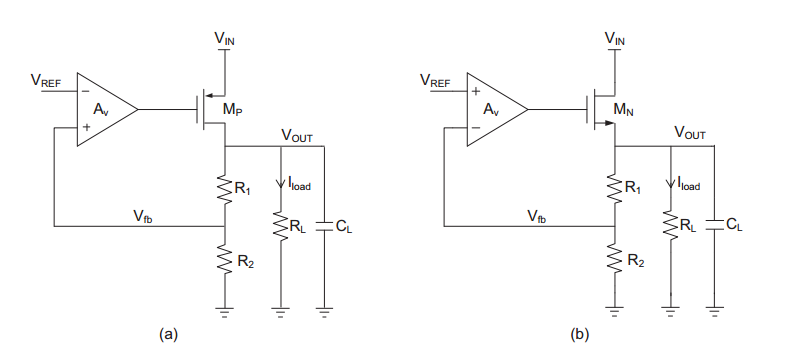
\includegraphics[keepaspectratio,alt={classical voltage reg topologies nmos and pmos pass devices}]{../theoretical_fundamentals/images/classical_voltage_reg_topologies_nmos_and_pmos_pass_devices.png}}
\caption{Classical Voltage Regulator Topology: a) with PMOS pass device
and b) with NMOS pass
device}\label{classical_voltage_reg_topologies_nmos_and_pmos_pass_devices}
\end{figure}

\subsection{Static/Steady-State
Parameters}\label{_staticsteady_state_parameters}

\subsubsection{Drop-out Voltage}\label{_drop_out_voltage}

The drop-out voltage is defined as the minimum voltage difference
between VIN and VOUT (Figure 2.1) to maintain an intended voltage
regulation {[}4\_yang\_li\_thesis{]}. A linear regulator which can
operate in low drop-out voltage regulation is commonly named as low
drop-out regulator (LDO). The application intended for the proposed
voltage regulator has quite a big dropout, that allows us to use an NMOS
pass device without a charge pump, as such it does not qualify it as a
Low-Dropout Regulator.

\subsubsection{Quiescent Current}\label{_quiescent_current}

The quiescent current (I\textsubscript{Q}) is defined as the total
current drawn by the voltage regulator from the preceding supply, minus
the current that flows to the load. In other words it's the current
consumed by the control circuits. The power efficiency η of a linear
regulator can be expressed in, where I\textsubscript{Load} is current
flowing into the load and V\textsubscript{dropout} is the dropout
voltage.

\[\eta = \frac{P_{delivered}}{P_{supplied}} = \frac{V_{out}I_{load}}{V_{in}(I_{load} + I_Q)}
= \left(1 - \frac{V_{dropout}}{V_{in}}\right)\frac{I_{load}}{(I_{load} + I_Q)}\]

\subsubsection{Line Regulation}\label{_line_regulation}

Line regulation measures a voltage regulator's ability to maintain a
stable output voltage \(V_{out}\) despite static or low-frequency
variations in its input supply voltage \(V_{in}\). It is quantitatively
defined as the ratio of the change in output voltage to the change in
input voltage:

\[\text{Line Regulation} = \frac{\Delta V_{out}}{\Delta V_{in}} = \frac{v_{out}}{v_{in}}\]

\emph{Note: This is also frequently expressed as a percentage of the
nominal output voltage per volt, i.e., \(\% / \text{V}\), or simply in
\(\text{mV}/\text{V}\).}

The input supply feeding the regulator is rarely perfectly stable. It
often fluctuates due to a combination of factors, such as:

\begin{itemize}
\item
  The line and load regulation limitations of the preceding supply
  regulator.
\item
  Thermal drift and bandgap reference inaccuracies.
\item
  Static offsets resulting from transistor mismatches.
\item
  AC ripple originating from upstream switching regulators or
  rectifiers.
\end{itemize}

Ideally, the regulated output voltage should remain constant at its
target value across the entire operating range of the input voltage.
This ideal behavior holds true until the input voltage drops too close
to the output voltage, reaching the "dropout" threshold. For an NMOS
pass-transistor topology, as \(V_{in}\) decreases toward this limit, the
gate-driving stage (often an error amplifier powered by \(V_{in}\) or a
charge pump) runs out of voltage headroom to sufficiently command the
NMOS gate. This pushes the NMOS pass element from its active
(saturation) region into the triode region, causing the regulator to
drop out of regulation.

However, even within the normal operating range, the output voltage is
not fully immune to input fluctuations. Due to the finite loop gain of
the feedback network, the output voltage varies slightly in response to
changes in the input supply.

Specifically, the closed-loop line regulation is determined by the
open-loop sensitivity of the regulator divided by the feedback loop
gain:

\[\left(\frac{\partial V_{out}}{\partial V_{in}}\right)_{\text{closed-loop}} \approx \frac{\left( \frac{\partial V_{out}}{\partial V_{in}} \right)_{\text{open-loop}}}{1 + T(s)}\]

where \(T(s)\) represents the loop gain of the regulation loop (the
product of the error amplifier gain, the pass element gain, and the
feedback factor).

In an open-loop condition, a change in \(V_{in}\) directly affects the
output through the finite output impedance (\(r_{ds}\)) and
channel-length modulation of the pass transistor, as well as through any
body effect (particularly in NMOS source followers). Because the loop
gain \(T(s)\) is finite, and further decreases at higher frequencies,
the error amplifier cannot completely suppress these perturbations,
leading to a measurable shift in \(V_{out}\) when \(V_{in}\) changes. To
achieve superior line regulation, the low-frequency gain of the error
amplifier must be maximised.

\paragraph{Small-Signal Analysis of the Line Regulation of a voltage
regulator with an NMOS Pass
device}\label{_small_signal_analysis_of_the_line_regulation_of_a_voltage_regulator_with_an_nmos_pass_device}

To establish a formal quantitative analysis of the line regulation for
an NMOS-based regulator, we evaluate its small-signal model. The
analysis starts from the regulator model of
\hyperref[classical_voltage_reg_topologies_nmos_and_pmos_pass_devices]{Classical
Voltage Regulator Topology: a) with PMOS pass device and b) with NMOS
pass device}(b). Let the transconductance of the NMOS pass transistor
\(M_N\) be \(g_{mn}\), its output resistance be \(r_{ds\_n}\), and the
open-loop voltage gain of the error amplifier be \(A_{OTA}\).

The feedback network consists of a resistive divider \(R_1\) and
\(R_2\), while \(R_L\) represents the load resistance. The small-signal
relationship describing the propagation of an input variation
\(\Delta V_{in}\) to the output variation \(\Delta V_{out}\) is given
by:

\[\left[ \left( -\Delta V_{out} \frac{R_2}{R_1 + R_2} A_{OTA} - \Delta V_{out} \right) g_{mn} + \frac{\Delta V_{in} - \Delta V_{out}}{r_{o,n}} \right] \left[ (R_1 + R_2) \parallel R_L \right] = \Delta V_{out}\]

By solving this equation for the transfer function
\(\Delta V_{out} / \Delta V_{in}\), the exact expression for the line
regulation of the NMOS regulator is derived as:

\[\frac{\Delta V_{out}}{\Delta V_{in}} = \frac{v_{out}}{v_{in}} = \frac{1}{\left(1 + \frac{R_2}{R_1 + R_2} A_{OTA}\right) g_{mn} r_{o,n} + \frac{r_{o,n}}{(R_1 + R_2) \parallel R_L} + 1}\]

Under typical operating conditions, the loop gain is high, and the
expression could be simplified to:

\[\frac{\Delta V_{out}}{\Delta V_{in}} = \frac{v_{out}}{v_{in}} \approx \frac{1}{\frac{R_2}{R_1 + R_2} A_{OTA} g_{mn} r_{o,n}}\]

\subsubsection{Physical Comparison: NMOS vs. PMOS
Regulators}\label{_physical_comparison_nmos_vs_pmos_regulators}

The simplified formulation reveals that the line regulation of the NMOS
regulator is inversely proportional to both the amplifier's open-loop
gain \(A_{OTA}\) and the intrinsic gain of the NMOS pass transistor,
\(g_{mn} r_{o,n}\).

Compared to a conventional PMOS-based regulator---which typically
exhibits a line regulation of approximately:

\[\left(\frac{\Delta V_{out}}{\Delta V_{in}}\right)_{\text{PMOS}} \approx \frac{1}{\frac{R_2}{R_1 + R_2} A_{OTA}}\]

the NMOS regulator improves line regulation performance by a factor of
\(g_{mn} r_{o,n}\).

This key performance advantage is physically intuitive when considering
the topology of the pass device. The NMOS pass transistor effectively
functions as a "cascode" transistor situated between the noisy input
supply \(V_{in}\) (connected to its drain) and the output node
\(V_{out}\) (connected to its source). Because any voltage variation
applied to the drain of a regulated NMOS transistor is inherently
shielded by the channel, its equivalent variation at the source node is
heavily attenuated by the transistor's intrinsic gain \(g_{mn} r_{o,n}\)
in addition to the closed-loop feedback gain \(A_{OTA}\).

\subsection{Load Regulation}\label{_load_regulation}

Load regulation measures a voltage regulator's ability to maintain a
stable output voltage in the presence of static or low-frequency
variations in the load current. It is mathematically defined as the
ratio of the static output voltage variation (\(\Delta V_{out}\)) to the
static load current change (\(\Delta I_{out}\) or \(\Delta I_{load}\multi-loop\)):

\[\text{Load Regulation} = \frac{\Delta V_{out}}{\Delta I_{load}} = \frac{v_{out}}{i_{load}}\]

This ratio essentially represents the closed-loop output impedance
(\(R_{out\_closed\_loop}\)) of the regulator. A lower closed-loop output
impedance corresponds to superior load regulation, meaning lower static
output voltage deviations due to varying load currents.

\subsubsection{Small-Signal Analysis of the NMOS
Regulator}\label{_small_signal_analysis_of_the_nmos_regulator}

To analyze the load regulation of the NMOS regulator quantitatively, we
utilize the small-signal representation based again on the regulator
model from
\hyperref[classical_voltage_reg_topologies_nmos_and_pmos_pass_devices]{Classical
Voltage Regulator Topology: a) with PMOS pass device and b) with NMOS
pass device}(b). In this model, \(A_{OTA}\) is the open-loop gain of the
error amplifier, \(g_{mn}\) is the transconductance of the NMOS pass
element, and \(I_{load}\) represents the load current flowing through
the load resistance \(R_L\).

When the load current changes by a small-signal amount
\(\Delta I_{load}\), it induces a corresponding shift in the output
voltage \(\Delta V_{out}\). The small-signal relationship describing the
impact of this load current variation on the output voltage is
formulated as:

\[\left( -\Delta V_{out} \frac{R_2}{R_1 + R_2} A_{OTA} - \Delta V_{out} \right) g_{mn} = \Delta I_{load}\]

By rearranging the terms to isolate the transfer function
\(\Delta V_{out} / \Delta I_{load}\), we obtain the closed-loop
expression:

\[\frac{\Delta V_{out}}{\Delta I_{load}} = -\frac{1}{\left( \frac{R_2}{R_1 + R_2} A_{OTA} + 1 \right) g_{mn}}\]

Under typical operating conditions where the loop gain is significantly
high (such that \(\frac{R_2}{R_1 + R_2} A_{OTA} \gg 1\)), this
expression simplifies to:

\[\frac{\Delta V_{out}}{\Delta I_{load}} \approx -\frac{1}{\frac{R_2}{R_1 + R_2} A_{OTA} g_{mn}}\]

The negative sign indicates that an increase in load current (current
drawn out of the regulator) causes a small, proportional drop in the
output voltage.

\subsubsection{Physical Intuition and Feedback
Mechanism}\label{_physical_intuition_and_feedback_mechanism}

The small-signal analysis demonstrates that the load regulation of the
NMOS regulator depends on both the amplifier open-loop gain
(\(A_{OTA}\)) and the transconductance of the NMOS pass device
(\(g_{mn}\)).

This dependency is directly linked to the properties of negative shunt
feedback:

\begin{enumerate}
\def\labelenumi{\arabic{enumi}.}
\item
  \textbf{Open-loop Output Impedance:} The pass device in an NMOS
  regulator behaves as a source follower. Looking into the source of the
  NMOS transistor, the open-loop output impedance is approximately:

  \[R_{out, ol} \approx \frac{1}{g_{mn}}\]
\item
  \textbf{Loop Gain:} The feedback loop consists of the resistor divider
  ratio \(\beta = R_2 / (R_1 + R_2)\), the error amplifier gain
  \(A_{OTA}\), and the pass-device source-follower gain (which is
  approximately unity). This yields a loop gain of:

  \[T \approx \frac{R_2}{R_1 + R_2} A_{OTA}\]
\item
  \textbf{Closed-loop Output Impedance:} The voltage-sensing
  shunt-feedback at the output node reduces the output impedance by a
  factor of \(1 + T\):

  \[R_{out, cl} = \frac{R_{out, ol}}{1 + T} \approx \frac{1/g_{mn}}{\frac{R_2}{R_1 + R_2} A_{OTA}} = \frac{1}{\frac{R_2}{R_1 + R_2} A_{OTA} g_{mn}}\]
\end{enumerate}

This derivation confirms that to minimize output voltage variations
under fluctuating load conditions, the design should focus on maximizing
both the error amplifier's open-loop gain (\(A_{OTA}\)) and the
transconductance (\(g_{mn}\)) of the NMOS pass element.

\subsection{Temperature Drift}\label{_temperature_drift}

Temperature variations directly affect the output voltage accuracy of a
linear regulator. The thermal stability of a regulator is quantified by
its temperature coefficient (\(TC\)), which is defined as the fractional
change of the output voltage in response to a change in temperature {[}5
G. Rincon-Mora, Analog IC Design with Low-Dropout Regulators{]}.
Typically expressed in percent per degree Celsius
(\(\%/^\circ\text{C}\)) or parts per million per degree Celsius
(\(\text{ppm}/^\circ\text{C}\)), the temperature coefficient is
mathematically defined as:

\[TC = \frac{1}{V_{out}} \frac{\Delta V_{out}}{\Delta T} = \frac{(\Delta V_{ref} + \Delta V_{os}) \left(\frac{V_{out}}{V_{ref}}\right)}{V_{out}\Delta T} = \frac{\Delta V_{ref} + \Delta V_{os}}{V_{ref}\Delta T}\]

Where:

\begin{itemize}
\item
  \(\Delta T\) represents the change in temperature.
\item
  \(\Delta V_{ref}\) represents the variation in the reference voltage
  over temperature.
\item
  \(\Delta V_{os}\) represents the variation in the error amplifier's
  input-referred equivalent offset voltage over temperature.
\end{itemize}

Based on the derivation above, the absolute value of the output voltage
cancels out. This indicates that the regulator's overall temperature
coefficient is independent of the target output voltage setting.
Instead, the thermal stability of the regulator is directly determined
by two primary components:

\begin{enumerate}
\def\labelenumi{\arabic{enumi}.}
\item
  \textbf{The reference voltage temperature coefficient:}
  \(\frac{\Delta V_{ref}}{V_{ref}\Delta T}\)
\item
  \textbf{The input-referred offset voltage drift scaled by the
  reference voltage:} \(\frac{\Delta V_{os}}{V_{ref}\Delta T}\)
\end{enumerate}

To minimize temperature drift in practical linear regulator designs, it
is necessary to utilize a highly stable bandgap reference with a low
temperature coefficient, alongside an error amplifier optimized to
minimize thermal offset drift (\(\Delta V_{os}/\Delta T\)) through a low
mismatch optimized input pair, high DC open-loop gain and layout
matching techniques.

\subsubsection{Minimizing Thermal Drift in Linear
Regulators}\label{_minimizing_thermal_drift_in_linear_regulators}

Achieving high-precision thermal performance in linear regulators
requires addressing both the primary reference voltage source and the
non-idealities of the feedback loop. This section examines the specific
design and layout techniques used to mitigate these thermal effects.

\subsubsection{Bandgap Reference (BGR) Temperature
Coefficient}\label{_bandgap_reference_bgr_temperature_coefficient}

The bandgap reference provides the baseline voltage \(V_{ref}\).
Standard bandgap circuits achieve first-order temperature cancellation
by summing two voltages with opposite thermal behaviors:

\begin{itemize}
\item
  \textbf{CTAT (Complementary-to-Absolute-Temperature):} The
  base-emitter voltage of a bipolar junction transistor (\(V_{BE}\))
  decreases linearly with temperature, typically at a rate of
  approximately:

  \[\frac{\partial V_{BE}}{\partial T} \approx -2 \, \text{mV}/^\circ\text{C}\]
\item
  \textbf{PTAT (Proportional-to-Absolute-Temperature):} The thermal
  voltage \(V_T = k_B T / q\) increases linearly with temperature,
  exhibiting a temperature coefficient of:

  \[\frac{\partial V_T}{\partial T} \approx +0.086 \, \text{mV}/^\circ\text{C}\]
\end{itemize}

By scaling and summing these two voltages, a first-order
temperature-compensated reference voltage of approximately
\(1.2 \, \text{V}\) (or lower for fractional bandgaps) is produced:

\[V_{ref}(T) = V_{BE}(T) + K \cdot V_T(T)\]

where \(K\) is a constant defined by transistor sizing and resistor
ratios. Even with this first-order compensation, residual second-order
temperature effects remain that influence the bandgap's temperature
coefficient.

\subsubsection{Mitigating Error Amplifier Offset
Drift}\label{_mitigating_error_amplifier_offset_drift}

Even with a perfectly stable reference, any thermal drift in the error
amplifier's input-referred offset voltage (\(\Delta V_{os}/\Delta T\))
propagates directly to the output. This offset is composed of both
random and systematic components.

\paragraph{Random Offset and Pelgrom's
Law}\label{_random_offset_and_pelgroms_law}

Random offset arises from local, microscopic variations in transistor
physical dimensions, doping concentrations, and oxide thicknesses. In
the input differential pair of the error amplifier, threshold voltage
(\(V_{th}\)) mismatch is the dominant driver of offset drift.

According to \textbf{Pelgrom's Law}, the standard deviation of threshold
voltage mismatch (\(\sigma_{\Delta V_{th}}\)) is inversely proportional
to the square root of the active gate area:

\[\sigma_{\Delta V_{th}} = \frac{A_{Vth}}{\sqrt{W \cdot L}}\]

where \(A_{Vth}\) is a technology-dependent constant, while \(W\) and
\(L\) represent the width and length of the input transistors.

To minimize random thermal drift:

\begin{itemize}
\item
  \textbf{Large Device Sizing:} Designers use large gate areas (high
  \(W \cdot L\)) for the input pair. Increasing the area averages out
  local channel fluctuations, lowering both the nominal offset and its
  corresponding drift over temperature.
\end{itemize}

\paragraph{Systematic Offset and High DC Open-Loop
Gain}\label{_systematic_offset_and_high_dc_open_loop_gain}

Systematic offset occurs due to circuit design asymmetries, such as
drain-to-source voltage (\(V_{DS}\)) imbalances in the input pair or
load current mirrors. Because these biases change dynamically with
temperature, they introduce systematic drift.

Maintaining a high DC open-loop gain (\(A_{OL}\)) in the error amplifier
minimizes this systematic drift by heavily attenuating closed-loop gain
errors:

\[\epsilon_{gain} \approx \frac{1}{1 + A_{OL}\beta}\]

A high \(A_{OL}\) ensures that the amplifier behaves closer to its
mathematical ideal, ensuring that thermal variations in internal node
voltages do not manifest as a shifting input-referred offset.

\subsection{Transient Response and Slew
Rate}\label{_transient_response_and_slew_rate}

The Slew Rate directly impacts the transient response of the voltage
regulator, which is crucial for maintaining the output voltage within
acceptable limits under varying load conditions. In automotive
applications, where power efficiency and reliability are paramount,
optimizing the Slew Rate can lead to improved performance and reduced
power consumption.

Usually, for a step in the output load current, from 0 to a maximum
value \(I_{load\_max}\), the maximum output voltage variation
\(\Delta V_{out\_max}\) can be expressed as:

\[\Delta V_{out\_max} = (\frac{1}{BW_{cl}} + \frac{\Delta V_{gate} \cdot C_{gate}}{I_{SR}})\cdot \frac{I_{load\_max}}{C_{load}}\]

At the first moment of the current step, the control loop has not had
time to react. The extra current demand, \(\Delta I_{load\_max}\), is
supplied entirely by the output capacitor, \(C_{load}\). This causes the
output voltage to start dropping at a rate:
\(\frac{\Delta I_{load\_max}}{C_{load}}\). The output voltage will stop
dropping at the instant when the power stage supplies exactly the same
value of the demanded load current. Until then, the loop will try to
react and restore the output voltage, but the response time is limited
by the loop bandwidth, \(BW_{cl}\). During this time, the output voltage
will have dropped by an amount:
\(\frac{\Delta I_{load\_max}}{C_{load} \cdot BW_{cl}}\). After the loop
starts to react, the gate voltage of the pass transistor will begin to
change. The time it takes for the gate voltage to change by the required
amount such as to supply the demanded load current can be written as:
\(t_{sr} = \frac{\Delta V_{gate}}{SR_{Gate}} = \frac{\Delta V_{gate} \cdot C_{gate}}{I_{SR}}\).

As can be seen from the equation the loop bandwidth and the slew rate of
the OTA play an essential role in shaping the transient response of the
voltage regulator.

If we consider the NMOS voltage regulator as a two-pole system with the
dominant pole at the power stage's node and the second pole at the
output node, the worst case stability scenario is at low load current
and high output capacitance. The value of the gate capacitor should be
chosen such that stability at the lowest required load current and
maximum load capacitance is ensured. From this design constraint, there
is an effective upper bound on the possible bandwidth of the control
loop.

The other parameter that we are free to tune is the Slew Rate of the
OTA. Indeed, increasing the Slew Rate will reduce the time it takes for
the gate voltage to change, thus improving the transient response of the
regulator.

\hyperref[loadJump_ota_model_linear_transientResponse_2u_vs_5u_Islew]{Load
jump response comparison between two OTA models with different Slew
Rates} shows the difference in transient response between two OTA models
with different Slew Rates. The OTA with a higher Slew Rate (5uA/V) shows
a faster recovery to the nominal output voltage after a load jump
compared to the OTA with a lower Slew Rate (2uA/V). This demonstrates
the importance of optimizing the Slew Rate in the design of voltage
regulators, especially in applications where rapid load changes are
expected.

\begin{figure}
\centering
\pandocbounded{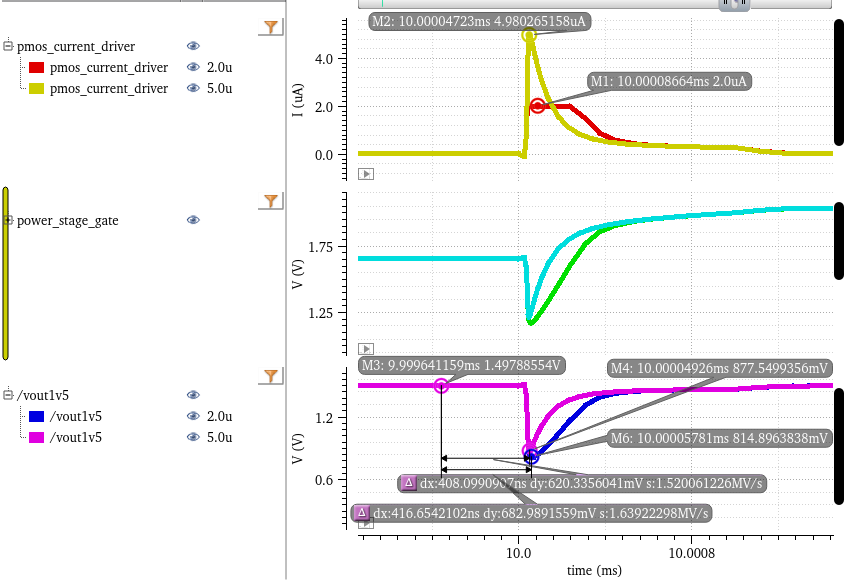
\includegraphics[keepaspectratio,alt={loadJump ota model linear char 2u vs 5u Islew}]{../theoretical_fundamentals/images/loadJump_ota_model_linear_char_2u_vs_5u_Islew.png}}
\caption{Load jump response comparison between two OTA models with
different Slew
Rates}\label{loadJump_ota_model_linear_transientResponse_2u_vs_5u_Islew}
\end{figure}

However, we must keep in mind the conditions under which eq. (1) was
derived and remains valid. The equation assumes that the output current
exhibits both a hard saturation on the bias current and a linear
dependence on the input differential voltage. Therefore, increasing the
Slew Rate requires more current from the OTA, which leads to increased
power consumption. Therefore, there is a trade-off between transient
response and power efficiency that must be carefully balanced in the
design of the voltage regulator, for class-A type OTAs.

For class AB OTAs, which typically exhibit a nonlinear relationship
between the output current and the input differential voltage, the
situation differs. In these devices, the slew rate can be enhanced
without significantly raising the quiescent current, improving the
transient response without a substantial power penalty.
\hyperref[dc_sweep_ota_model_linear_vs_quadratic]{DC sweep of the output
current injected by the OTA block for a decrease in its negative input
voltage} illustrates the differing output current behaviors of a linear
and a quadratic OTA model. The linear model demonstrates hard saturation
at the 2 µA bias current when the output voltage drops below 1 V.
Conversely, the quadratic model initially presents a lower slope,
resulting in a lower transconductance for minor voltage deviations, but
this slope increases rapidly. Consequently, its output current overtakes
that of the linear model for voltages below 1.025 V. (It should be noted
that no current saturation was incorporated into this simplified
quadratic model). Therefore, boosting an OTA's slew rate via a nonlinear
stage can improve transient behavior and power efficiency, even if the
unity-gain bandwidth is held constant.

\begin{figure}
\centering
\pandocbounded{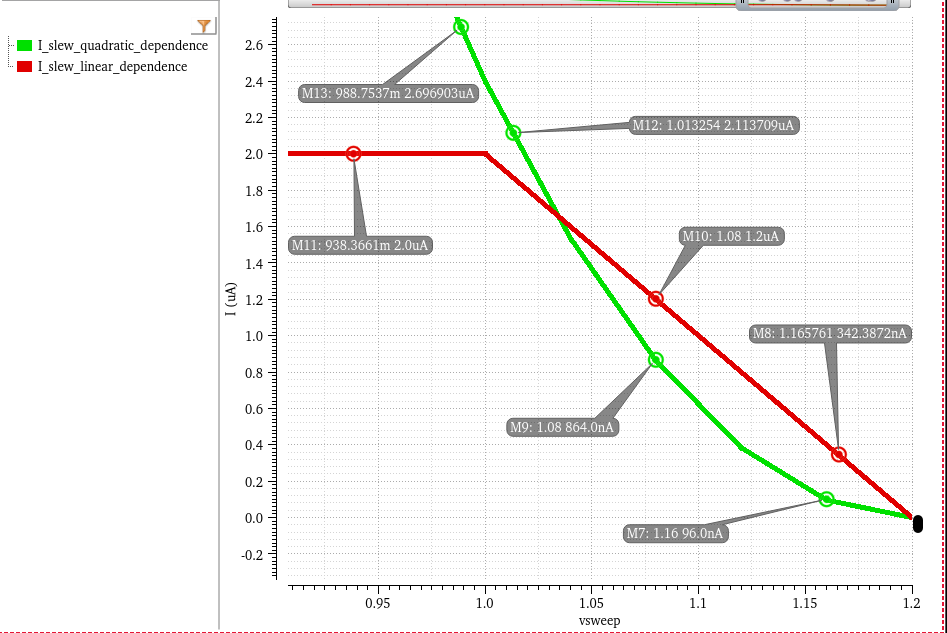
\includegraphics[keepaspectratio,alt={dc sweep slew rates linear vs quadratic dependence}]{../theoretical_fundamentals/images/dc_sweep_slew_rates_linear_vs_quadratic_dependence.png}}
\caption{DC sweep of the output current injected by the OTA block for a
decrease in its negative input
voltage}\label{dc_sweep_ota_model_linear_vs_quadratic}
\end{figure}

The resulting transient response of both ota models to a load jump is
shown in \hyperref[loadJump_ota_model_linear_vs_quadratic]{Load jump
response comparison between one OTA model with linear Iout dependence on
input differential voltage and Slew Rate cap and another OTA model with
quadratic Iout dependence on input differential voltage}. The OTA with
the nonlinear output current dependence on the input differential
voltage shows a smaller undershoot and a faster recovery to the nominal
output voltage after a load jump compared to the OTA with a linear
output current dependence, even though both OTAs have the same
unity-gain bandwidth. This demonstrates that optimizing the Slew Rate
through nonlinear stages can significantly enhance the transient
response of voltage regulators without necessarily increasing power
consumption.

\begin{figure}
\centering
\pandocbounded{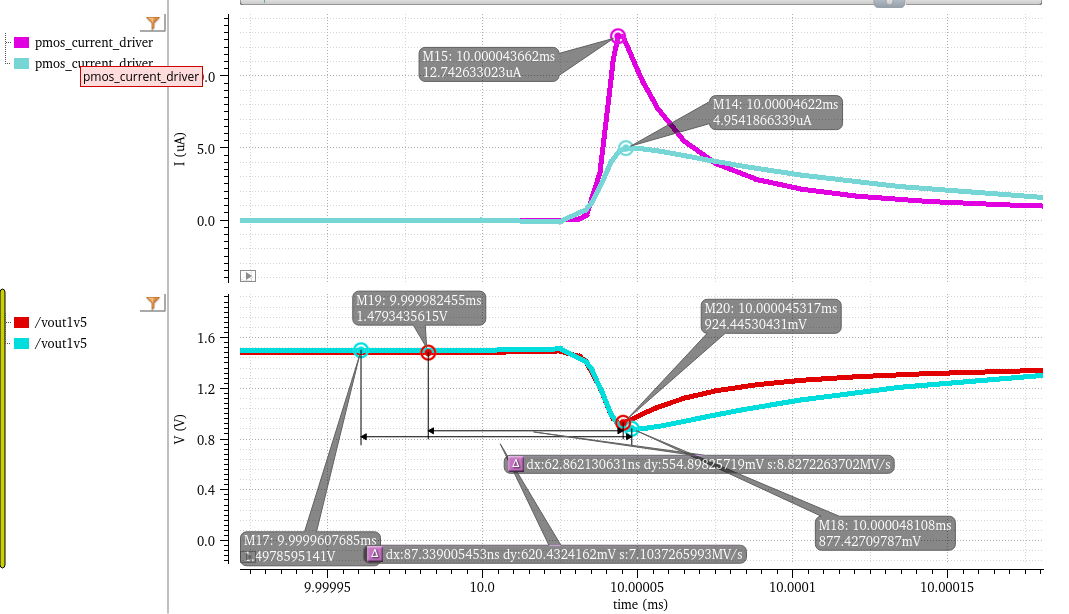
\includegraphics[keepaspectratio,alt={loadJump ota model linear vs quadratic dependence}]{../theoretical_fundamentals/images/loadJump_ota_model_linear_vs_quadratic_dependence.png}}
\caption{Load jump response comparison between one OTA model with linear
Iout dependence on input differential voltage and Slew Rate cap and
another OTA model with quadratic Iout dependence on input differential
voltage}\label{loadJump_ota_model_linear_vs_quadratic}
\end{figure}

\subsection{Stability Analysis of Dual-Loop
Systems}\label{_stability_analysis_of_dual_loop_systems}

While stability analysis of circuits with only one feedback loop is well
covered by the classical feedback theory and several methods are
available for deriving the phase- and gain-margins associated with the
circuit return ratio {[}cite Bode, Rosenstark, Neag{]}, however
extending this approach to circuits with multiple feedback loops is not
straightforward.

\begin{figure}
\centering
\pandocbounded{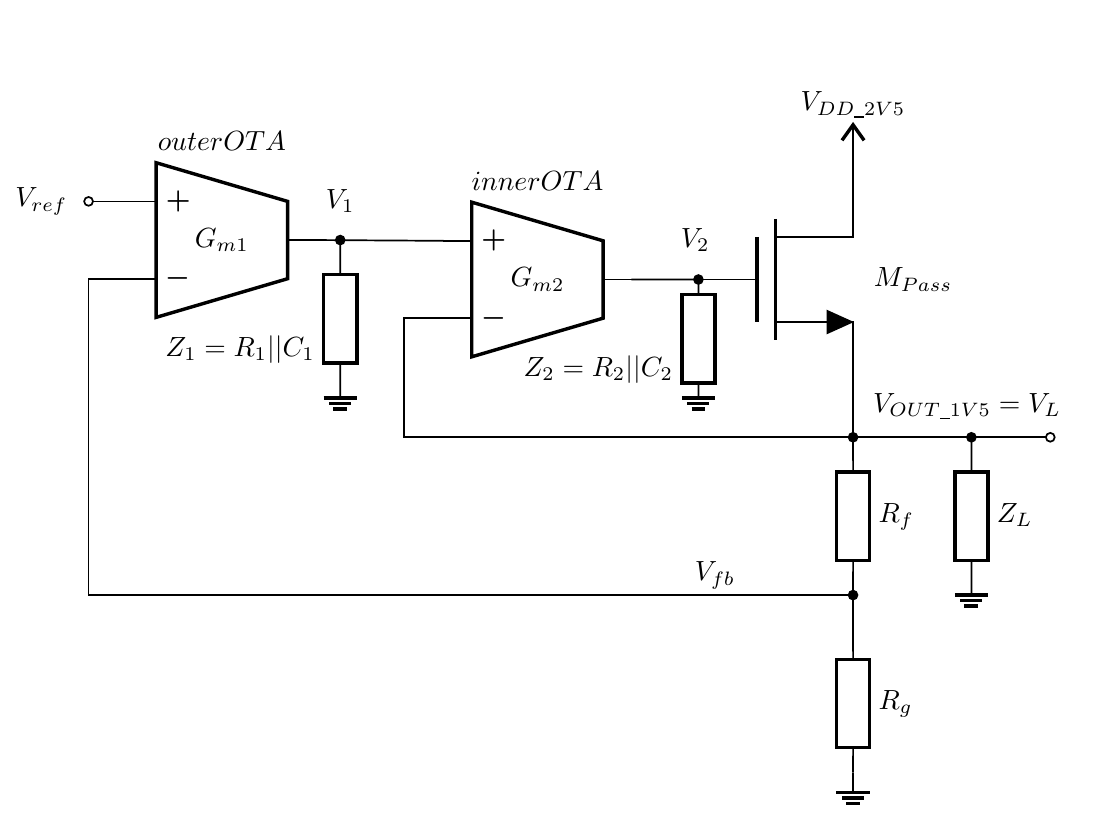
\includegraphics[keepaspectratio,alt={Dual Loop Regulator Architecture}]{../theoretical_fundamentals/images/dualLoop_stability_analysis/dual_loop_reg_model.png}}
\caption{Dual Loop Regulator
Architecture}\label{fig:dual_loop_reg_model}
\end{figure}

\subsubsection{Analysing the Dual-Loop Voltage Regulator's stability
using the classical feedback
theory}\label{sec:stb_using_classical_fb_theory}

Nonetheless, we can analyse the dual-loop system by breaking the inner
loop first and then evaluating the outer loop with the inner loop
replaced with its closed-loop equivalent as stated by classical feedback
theory. The innerloop comprises the path through the \(innerOTA\) and
the NMOS power stage and thus it has two poles, one dominated by the
node connected to the gate of the power stage and one dominated by the
output node of the regulator.

\begin{equation}
    T_{inner} = \frac{G_{m2}R_2}{(1+sR_2C_2)(1+ s \cdot C_L/g_{mp})}
    \label{eq:T_inner}
\end{equation}

The dual-loop system is stable if both the inner loop and the equivalent
single-loop system meet the usual stability requirements {[}Grajdeanu \&
all, 2022{]}. Let's set the condition that the second pole of the inner
loop is pushed up above the unity-gain frequency of that loop:

\begin{gather}
    UGF_{inner}  \ll f_{p\_out} \nonumber \\
    \frac{G_{m2}R_2}{R_2C_2}    \ll \frac{1}{C_L/g_{mp}} \implies \frac{G_{m2}}{C_2}    \ll \frac{g_{mp}}{C_L} \label{eq:classical_output_pole_constraint}
\end{gather}

Replacing the inner feedback loop by its closed loop equivalent we
obtain:

\begin{gather}
    H_{inner} = \frac{T_{inner}}{1 + T_{inner}} = \frac{\frac{G_{m2}R_2}{(1+sR_2C_2)(1+s/gmp \cdot C_L)}}{1+\frac{G_{m2}R_2}{(1+sR_2C_2)(1+s/gmp \cdot C_L)}}
    \\ = \frac{G_{m2}R_2}{(1+sR_2C_2)(1+s/gmp \cdot C_L) + G_{m2}R_2} \\
    \approx \frac{G_{m2}R_2}{(1+sR_2C_2) + G_{m2}R_2}
    \\ = \frac{1}{s\frac{C_2}{G_{m2}} + \frac{1}{G_{m2}R_2} + 1}
\end{gather}

As we can see, the equivalent closed-loop block of the inner feedback
loop is a unity gain low pass filter, with the first pole placed at
\(f = \frac{G_{m2}}{2 \pi C_2}\).

The loop gain of the entire regulator is now given by the product of
\(H_{inner}\) and the transmittance of the remaining circuitry, the
feedback resistive divider and \(G_{m1}\) \& \(Z_1\). To ensure the
stability of this loop (and allow for enough margin, considering the
gain peaking the inner loop may introduce), we impose the condition that
the UGF of \(T_{reg}\) is smaller than the closed-loop bandwidth of
\(H_{inner}\).

\begin{gather}
    T_{reg} = T_{outer} \cdot H_{inner} = \nonumber \\
    = \frac{G_{m1}fR_1}{1+sR_1C_1} \cdot \frac{1}{s\frac{C_2}{G_{m2}} + \frac{1}{G_{m2}R_2} + 1} \nonumber \\
    \frac{G_{m1}f}{C_1} \ll \frac{G_{m2}}{C_2} \label{eq:classical_treg_ugf_constraint}
\end{gather}

\subsection{Stability Analysis of Multi-Loop Systems using Signal Flow
Graphs and Driving Point
Impedance}\label{_stability_analysis_of_multi_loop_systems_using_signal_flow_graphs_and_driving_point_impedance}

Signal Flow Graphs (SFGs) offer a powerful alternative to characterize
linear circuit networks, as they automatically include all loading
effects at the input and output ports in the analysis without ever
requiring the loop to be physically broken {[}b1{]}.

The technique of Driving Point Impedance (DPI) analysis, introduced by
Ochoa {[}b1{]}, provides a systematic methodology for translating a
circuit schematic directly into an SFG. It is based on the
transformation of circuit nodes to their Norton equivalent
representations and the sequential application of superposition. The
resulting SFG alternates between two types of nodes: short-circuit
currents (\(I_{sc}\)) and node voltages (\(v\)). Active
transconductances (like \(g_m\)) act as directed branches that inject
current into the \(I_{sc}\) nodes, while the driving point impedances
(\(Z_{DP}\)) at each node convert these short-circuit currents back into
node voltages.

This graphical representation mirrors the Modified Nodal Analysis (MNA)
matrix equation {[}b2{]}:

\begin{equation}
    \mathbf{I} = \mathbf{Y} \cdot \mathbf{v}
    \label{eq:MNA_matrix}
\end{equation}

where \(\mathbf{Y}\) is the nodal admittance matrix, \(\mathbf{v}\) is
the vector of node voltages, and \(\mathbf{I}\) is the vector of
independent current sources.

Once the SFG is generated, Mason's Gain Formula provides a general
method for evaluating the transfer function between any two nodes. A
critical parameter in Mason's formula is the graph determinant,
\(\Delta\).

The roots of the characteristic equation \(\Delta = 0\) rigorously
define the closed-loop system's natural frequencies (poles).

While \(\Delta\) perfectly characterizes the closed-loop system,
directly extracting the open-loop gain in a multi-loop circuit requires
separating the main feedback loop from intrinsic local minor loops (like
parasitic capacitances or Early effect impedances). This requires the
application of Bode's Return Difference framework, which is discussed in
the next section.

Applying Ochoa's DPI technique to the dual-loop regulator in Fig.
\hyperref[fig:dual_loop_reg_model]{Dual Loop Regulator Architecture}
yields the SFG shown in Fig. \hyperref[fig:signalFlowGraph]{Signal Flow
Graph} with all local feedback loops included, which serves as the
foundation for the analytical loop gain extraction.

\begin{figure}
\centering
\pandocbounded{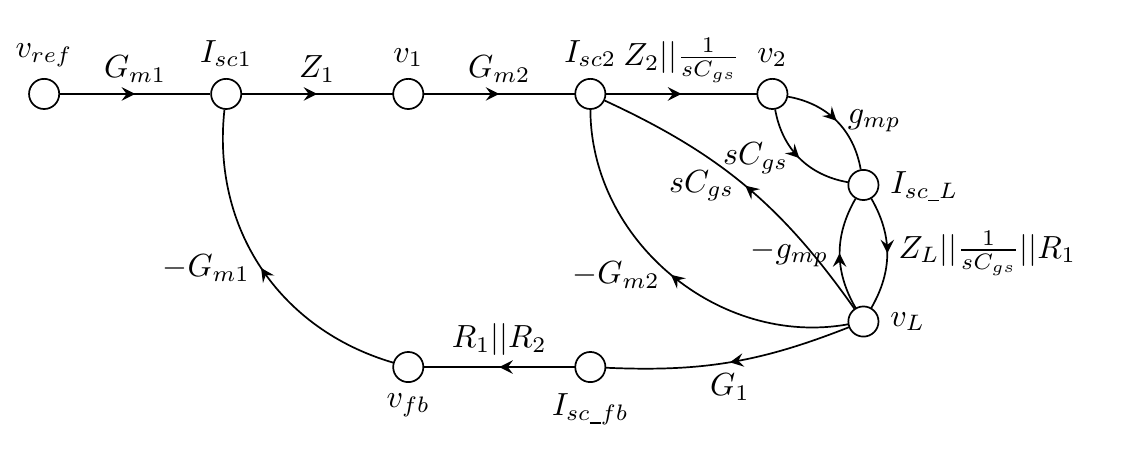
\includegraphics[keepaspectratio,alt={Signal Flow Graph}]{../theoretical_fundamentals/images/dualLoop_stability_analysis/signal_flow_graph.png}}
\caption{Signal Flow Graph}\label{fig:signalFlowGraph}
\end{figure}

\subsubsection{Analysing the Dual-Loop Voltage Regulator's stability
using SFGs and DPI}\label{sec:stb_using_sfg_and_dpi}

These circuit analysis techniques having been used for the VREG in Fig
\hyperref[fig:dual_loop_reg_model]{Dual Loop Regulator Architecture},
give rise to the SFG in Fig \hyperref[fig:signalFlowGraph]{Signal Flow
Graph} and lead to the following loop gain equation:

\begin{gather}
    T_{reg}(s) \approx \frac{G_{m2}R_2(1+G_{m1}R_1f)(1+s\frac{C_1}{G_{m1}f})(1+s\frac{C_{GS}}{g_{mp}})}{(1+sR_2C_2)(1+sR_1C_1)(1+s\frac{C_L}{g_{mp}})} - \nonumber\\
    - \frac{(1+s\frac{C_{GS}}{g_{mp}})sC_{GS}R_2}{(1+sR_2C_2)(1+s\frac{C_L}{g_{mp}})} \label{eq:T_reg_sfg}
\end{gather}

Eq. (\(\ref{eq:T_reg_sfg}\)) indicates a three pole system with a pole
associated with each of the three nodes denoted in
\hyperref[fig:dual_loop_reg_model]{Dual Loop Regulator Architecture},
the DC loop gain determined by the voltage gains of the two OTAs within
the two signal paths and a zero that appears due to the feedforwarding
action of the inner loop on the outer loop. Another zero appears because
of the \(C_{GS}\) of the power stage. That same parasitic capacitance,
if viewed bilaterally, yields a rhp pole, as indicated by the negative
term seen in (\(\ref{eq:T_reg_sfg}\)). The following inequalities turn
into design guidelines:

To maintain stability, we need to place the following constraints:

The first zero in the transfer function must occur before the unity gain
frequency, where the UGF has been computed as of a two-pole system with
no dominant pole:

\begin{equation}
    \frac{1+G_{m1}R_1f}{R_1C_1} < \sqrt{\frac{G_{m2}(1+G_{m1}R_1f)}{R_1C_1C_2}} \approx> \frac{G_{m1}f}{C_1} < \frac{G_{m2}}{C_2}
    \label{eq:zero_frequency_condition}
\end{equation}

We recognize this inequality also from
(\(\ref{eq:classical_treg_ugf_constraint}\)).

Last but not least, to ensure a suitable phase margin, the pole
associated with the output node should be pushed up in frequency at
least a decade above the unity gain bandwidth of the system:

\begin{equation}
    \frac{g_{mp}}{C_L} \gg \sqrt{\frac{G_{m2}(1+G_{m1}R_1f)}{R_1C_1C_2}}
    \label{eq:sfg_output_pole_constraint}
\end{equation}

Making use of the constraint obtained from
(\(\ref{eq:sfg_output_pole_constraint}\)), and knowing that

\begin{equation}
    \sqrt{\frac{G_{m2}(1+G_{m1}R_1f)}{R_1C_1C_2}} < \sqrt{(\frac{G_{m2}}{C_2})^2}
\end{equation}

We can obtain a more restrictive constraint, that corresponds to
(\(\ref{eq:classical_output_pole_constraint}\)), obtained using the
classical feedback theory approach:

\begin{equation}
    \frac{g_{mp}}{C_L} \gg \frac{G_{m2}}{C_2}
    \label{eq:output_pole_constraint}
\end{equation}

\subsection{Computing the Loop Gain of a Multi-Loop Feedback System
Numerically using Standard SPICE
Simulators}\label{sec:loop_gain_from_mna_matrices}

\subsubsection{Modified Nodal Analysis
(MNA)}\label{_modified_nodal_analysis_mna}

In a small-signal AC analysis, a linear or linearized circuit is
represented by its Admittance Matrix \(\mathbf{Y}(s)\). The relationship
between the node voltages \(\mathbf{v}(s)\) and the independent current
sources \(\mathbf{J}(s)\) is given by:

\begin{equation}
    \mathbf{Y}(s)\mathbf{v}(s) = \mathbf{J}(s)
    \label{eq:mna_equation}
\end{equation}

The matrix \(\mathbf{Y}(s)\) can be decomposed into a real conductance
matrix \(\mathbf{G}\) and a capacitance matrix \(\mathbf{C}\):

\begin{equation}
    \mathbf{Y}(s) = \mathbf{G} + s\mathbf{C}
    \label{eq:Y_decomposition_into_G_and_C}
\end{equation}

\subsubsection{Deriving the SFG Adjacency
Matrix}\label{_deriving_the_sfg_adjacency_matrix}

A Signal Flow Graph maps a system into the state-space-like topological
form:

\begin{equation}
    \mathbf{v} = \mathbf{A}\mathbf{v} + \mathbf{B}\mathbf{u}
\end{equation}

where \(\mathbf{A}\) is the Adjacency Matrix (branch gains between
dependent nodes), \(\mathbf{u}\) is the vector of external inputs, and
\(\mathbf{B}\) is the input coupling matrix.

To transform the MNA equation into the SFG format, we split
\(\mathbf{Y}\) into its diagonal components (\(\mathbf{Y}_{diag}\)) and
off-diagonal components (\(\mathbf{Y}_{off}\)):

\begin{equation}
    (\mathbf{Y}_{diag} + \mathbf{Y}_{off})\mathbf{v} = \mathbf{J} \implies
    \mathbf{Y}_{diag}\mathbf{v} = -\mathbf{Y}_{off}\mathbf{v} + \mathbf{J}
\end{equation}

By multiplying both sides by the inverse of the diagonal matrix
(\(\mathbf{Y}_{diag}^{-1}\)), we isolate \(\mathbf{v}\):

\begin{equation}
    \mathbf{v} = \underbrace{(-\mathbf{Y}_{diag}^{-1} \mathbf{Y}_{off})}_{\mathbf{A}} \mathbf{v} + (\mathbf{Y}_{diag}^{-1}) \mathbf{J}
\end{equation}

In standard nodal analysis, the independent driving vector
\(\mathbf{J}\) represents injected node currents. If the system's actual
external inputs are voltages (e.g., a reference voltage \(v_{ref}\)),
they manifest as currents injected into the nodes via transconductances
or admittances. We can map these voltage inputs (\(\mathbf{v}_{in}\)) to
injected currents via an input transconductance matrix
\(\mathbf{G}_{in}\):

Substituting this back yields the exact SFG state formulation:

\begin{equation}
    \mathbf{v} = \underbrace{(-\mathbf{Y}_{diag}^{-1} \mathbf{Y}_{off})}_{\mathbf{A}} \mathbf{v} + \underbrace{(\mathbf{Y}_{diag}^{-1}\mathbf{G}_{in})}_{\mathbf{B}} \underbrace{\mathbf{v}_{in}}_{\mathbf{u}}
\end{equation}

Thus, the exact Signal Flow Graph Adjacency Matrix is defined as:

\begin{equation}
    \mathbf{A}(s) = -\mathbf{Y}_{diag}^{-1}(s) \mathbf{Y}_{off}(s)
    \label{eq:A_built_by_admittance_matrix}
\end{equation}

Physically, the element \(A_{ij}\) represents the transconductance from
node \(j\) to node \(i\) multiplied by the total self-impedance at node
\(i\) (\(Z_{ii} = 1/Y_{ii}\)). This is the fundamental definition of a
branch gain in an SFG.

Beginning from the \(\mathbf{G}\) and \(\mathbf{C}\) matrices obtained
from a DCOP simulation (\(\ref{eq:Y_decomposition_into_G_and_C}\)), one
can build the adjacency matrix \(\mathbf{A}\) using
(\(\ref{eq:A_built_by_admittance_matrix}\)).

Then, using Mason's Gain Formula in matrix form, we can obtain the
global graph determinant \(\Delta\):

\begin{equation}
    \Delta = \det(\mathbf{I} - \mathbf{A}) = 1 - \sum L_i + \sum L_i L_j - \dots
\end{equation}

The global determinant \(\Delta\) encompasses \emph{all} loops in the
network, including the minor local loops intrinsic to active devices
(such as diode connections, Early effect impedances, and parasitic
capacitances). Consequently, these local loops mathematically inflate
the global determinant, obscuring the gain of the main feedback loop
{[}Middlebrook, International Journal of Circuit Theory and
Applications, 1998{]}.

To isolate the loop gain of the main feedback loop---what a circuit
designer actually cares about---we must invoke Bode's Return Ratio
theorem {[}Bode, Network Analysis and Feedback Amplifier Design,
1945{]}. Bode defined the Return Difference \(F\) with respect to a
chosen reference parameter \(W\) as the ratio of the total network
determinant \(\Delta\) to the "dead-system" determinant \(\Delta^0\):

\begin{equation}
    F = 1 + T = \frac{\Delta}{\Delta^0}
\end{equation}

In Bode's framework, \(W\) is a specific controlled source, typically
the \(g_m\) of an active device from the loop's forward gain. Setting
\(W = 0\) disconnects that source, so current no longer flows from the
drain to the source when the gate is driven. This is the active element
that vanishes to produce \(\Delta^0\), breaking the main loop while
leaving all passive loading and local minor loops perfectly intact.

In the MNA and SFG picture, this parameter \(W = g_m\) enters the
admittance matrix \(\mathbf{Y}\) as an off-diagonal entry,
\(\mathbf{Y}_{drain, gate} = g_m\). When transformed into the SFG
adjacency matrix using (\(\ref{eq:A_built_by_admittance_matrix}\)), it
becomes a directed SFG branch:

\begin{equation}
    \mathbf{A}_{drain\_gate} = -\frac{g_m}{\mathbf{Y}_{drain\_drain}}
\end{equation}

Setting \(W = g_m = 0\) to find the return ratio is therefore exactly
equivalent to zeroing that single SFG branch entry. By constructing a
modified adjacency matrix \(\mathbf{A}^0\) where this specific element
is zeroed out, we obtain the dead-system determinant
\(\Delta^0 = \det(\mathbf{I} - \mathbf{A}^0)\).

Therefore, the exact, loading-accurate loop gain \(T\) can be
numerically extracted directly from the circuit matrices as:

\begin{equation}
    T = \frac{\det(\mathbf{I} - \mathbf{A})}{\det(\mathbf{I} - \mathbf{A}^0)} - 1
\end{equation}

This matrix formulation strictly separates the principal loop gain from
local minor loops while preserving all complex loading effects unaltered
{[}Hurst, IEEE Transactions on Circuits and Systems II, 1991{]}.

\section{Implementation}\label{_implementation}

\subsection{Dual Loop Architecture}\label{_dual_loop_architecture}

To be able to improve on both static precision and dynamic performance,
a dual loop architecture was chosen: The outer loop was optimized for
high DC gain through a double-cascoded symmetrical OTA with an input
differential pair sized for low mismatch. {[}During steady‑state
operation, the high gain of the symmetrical outer OTA dominates the CCII
inner feedback loop, allowing the 1.5 V regulator to achieve under 2\%
precision in MC300 simulations.{]} To maintain optimal transient
performance, high DC gain and current efficiency, a biasing circuitry
with a PTAT component and an adaptive component that increases with load
current has been used.

\begin{figure}
\centering
\pandocbounded{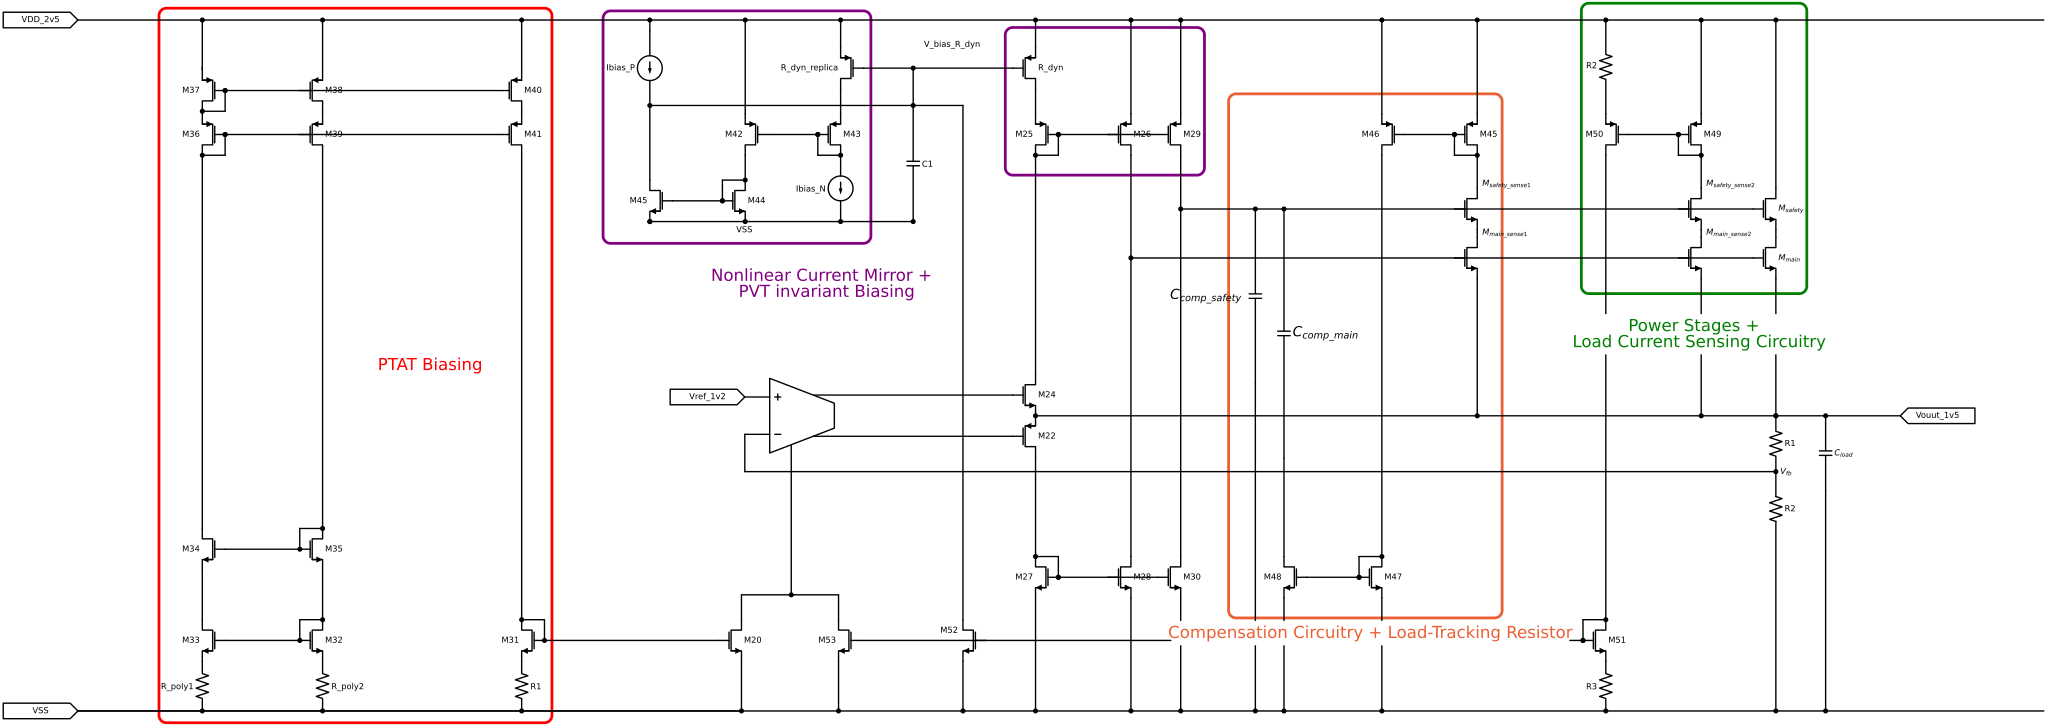
\includegraphics[keepaspectratio]{../implementation/images/1v5reg_block_diagram_1v5_reg.pdf}}
\caption{1V5 Voltage Regulator with Dual Loop Architecture}
\end{figure}

\subsection{Inner OTA Design and Slew Rate
Enhancement}\label{_inner_ota_design_and_slew_rate_enhancement}

For the Inner OTA a second generation current conveyor (CCII) was
chosen. The design mirrors the bipolar variant of Fabre {[}A Precise
Macromodel for Second Generation Current Conveyors Alain Fabre{]}
{[}Translinear current conveyors implementation Fabre{]}, using the same
translinear loop as its core. This design was chosen over the Barthelemy
variant {[}Barthelemy H (1997) Low-output-impedance class AB bipolar
voltage buffer{]} for its better quiescent current control over PVT.

The CCII has its Y voltage input is driven by the symmetrical outer OTA,
while its X current input is directly connected to the regulator output.
Owing to its simplicity, class AB behavior, and current feedback
operation, the CCII inner loop can be optimized for wide bandwidth and
high slew rate, allowing it to take over the system response during
transient events.

\begin{figure}
\centering
\pandocbounded{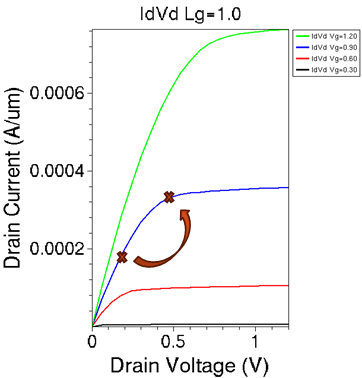
\includegraphics[keepaspectratio,alt={nonlinear currentMirror behaviour explanation using id vds graph}]{../implementation/images/nonlinear_currentMirror_behaviour_explanation_using_id_vds_graph.png}}
\caption{}
\end{figure}

Furthermore, a nonlinear PMOS current mirror that exploits the
transition from the triode region to saturation of a resistor-emulating
PMOS {[}4 - J. A. Galan, A. J. Lopez-Martin, R. G. Carvajal, J.
Ramirez-Angulo and C. Rubia-Marcos, "Super Class-AB OTAs With Adaptive
Biasing and Dynamic Output Current Scaling," {]} has been used to
further increase the positive slew rate of the inner OTA, ensuring 221mV
undershoots in full load jumps between 100nA and 10mA over PVT. R\_dyn
is biased at the edge of the triode region in steady state, but when a
sufficiently high current flows through M24 during a transient
undershoot event, R\_dyn will enter the saturation region to reach an
operating point with a higher drain current, but with the same VGS .
This mirrors gliding up the Y-axis of the ID/VDS graph of a MOSFET. A
slew rate comparison between a current conveyor with a classical and a
nonlinear current mirror is shown in Fig. 2. The regulation loop
response to a load jump from 100nA to 10mA with the two aforementioned
current mirrors is also shown in Fig. 3.

\subsection{Outer OTA Design and Loop
Stability}\label{_outer_ota_design_and_loop_stability}

The outer OTA is a double-cascoded symmetrical OTA with an input
differential pair sized for low mismatch biased in the subthreshold
region. The design of the outer OTA was optimized for high DC gain,
which is essential for achieving high precision in the voltage
regulator. The symmetrical architecture of the OTA helps to minimize
offset while the double-cascoding technique allows for a significant
increase in gain without sacrificing bandwidth. The single-stage
topology was chosen to minimize the quiescent current and the number of
poles in the system, thus improving stability margins.

\subsection{PTAT Current reference}\label{_ptat_current_reference}

\begin{figure}
\centering
\pandocbounded{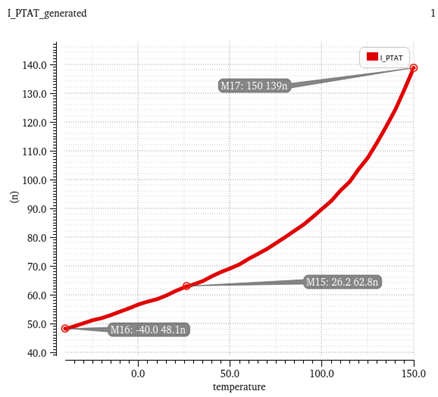
\includegraphics[keepaspectratio,alt={generated ptat current over temp}]{../implementation/images/generated_ptat_current_over_temp.png}}
\caption{}
\end{figure}

\subsection{Initial PTAT current reference
design}\label{_initial_ptat_current_reference_design}

The PTAT biasing circuitry is based on the classical ΔVGS PTAT core. The
extra resistor R\_poly2 has a PTAT behaviour, just like R\_poly1, but it
has a greater variance with temperature. In this way, the output PTAT
bias current has a lower process corner dependence.

\subsection{Improved PTAT current reference
design}\label{_improved_ptat_current_reference_design}

\begin{figure}
\centering
\pandocbounded{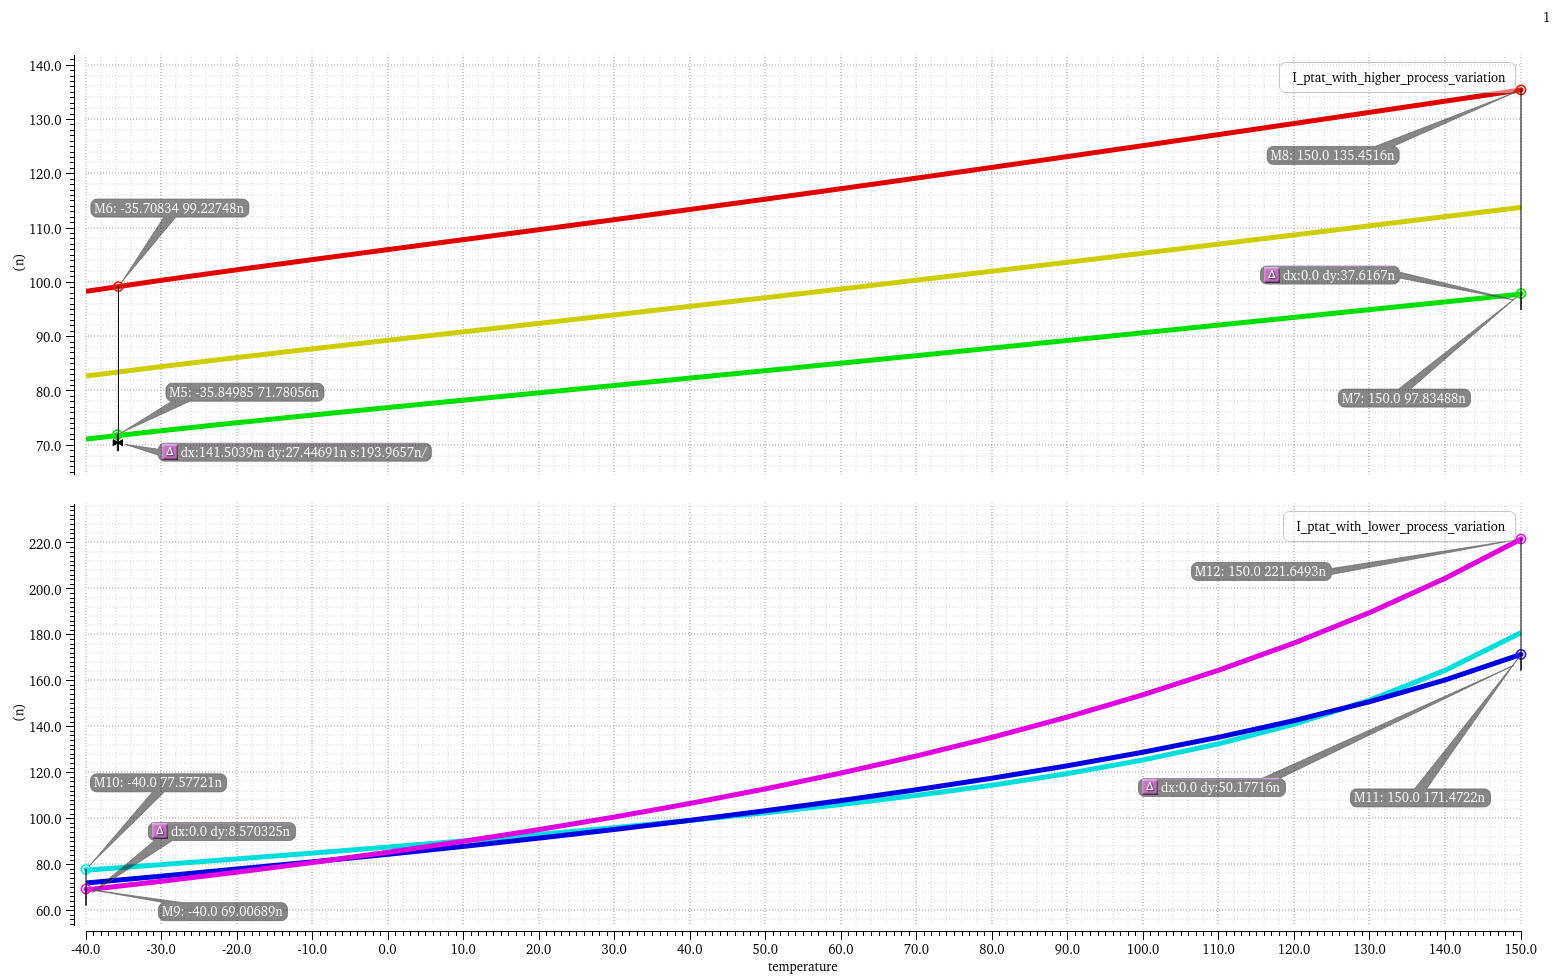
\includegraphics[keepaspectratio,alt={ptat current references comparison}]{../implementation/images/ptat_current_references_comparison.png}}
\caption{PTAT Current References Comparison}
\end{figure}

\subsection{Adaptive Biasing}\label{_adaptive_biasing_2}

\begin{figure}
\centering
\pandocbounded{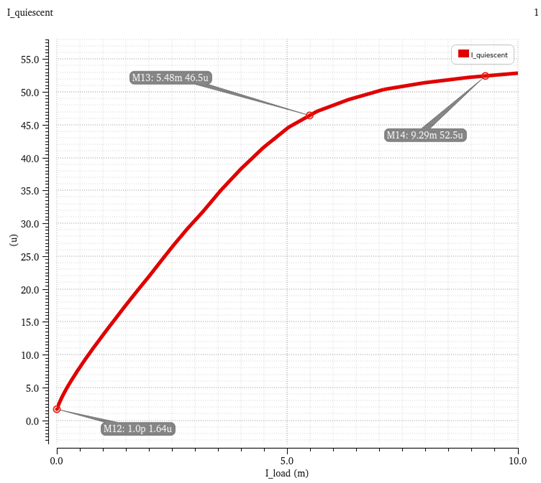
\includegraphics[keepaspectratio,alt={quiescentCurrent variation vs loadCurrent}]{../implementation/images/quiescentCurrent_variation_vs_loadCurrent.png}}
\caption{}
\end{figure}

The adaptive biasing current keeps the regulator's efficiency high at
minimum loads and increases the Unity Gain frequency, and Stability
margins at higher loads. It also allows the outer loop gain to surpass
80dB DC loop gain above 200 uA and 90dB above 2mA. With the help of a
variable resistor, implemented through M48, that generates a
load-tracking zero, stability is ensured for loads between 1u and 10mA
and 0 and 10nF, load current and capacitance, respectively.

\section{Experimental Results}\label{_experimental_results}

\subsection{VREG Startup and Disable}\label{_vreg_startup_and_disable}

\begin{figure}
\centering
\pandocbounded{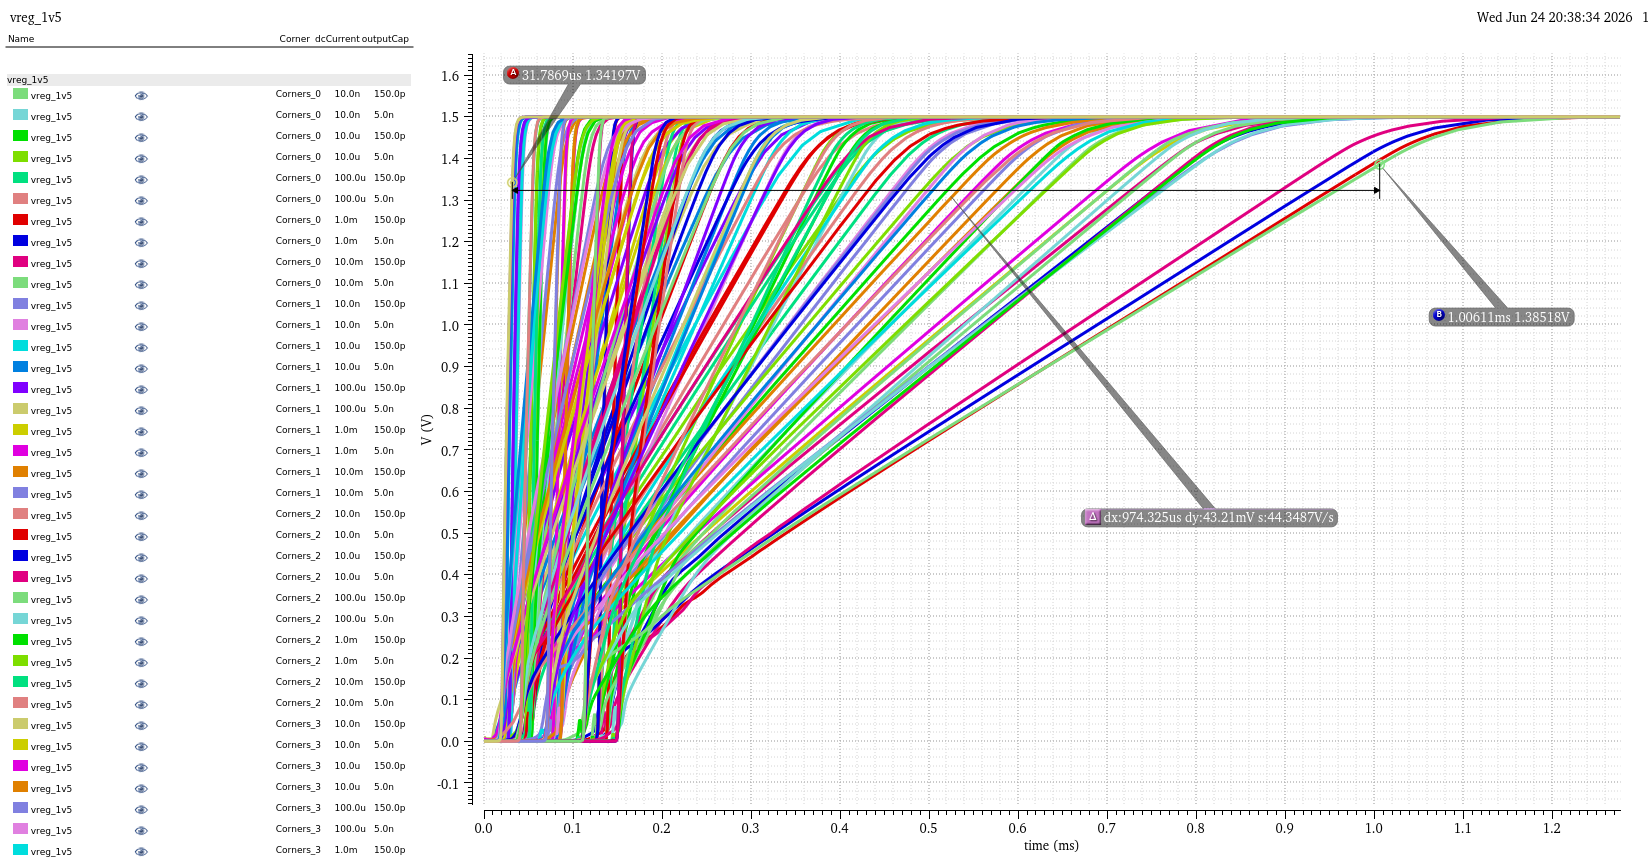
\includegraphics[keepaspectratio,alt={reg1v5 startup pvt cload 150p 5n iload 10n 10m sweep}]{../experimental_results/images/reg1v5_startup_pvt_cload_150p_5n_iload_10n_10m_sweep.png}}
\caption{Startup Behaviour of the 1.5V Regulator over PVT with 150pF and
5nF Load Capacitance and Load Current Sweep from 10nA to
10mA}\label{reg1v5_startup_pvt_cload_150p_5n_iload_10n_10m_sweep}
\end{figure}

As can be seen from
\hyperref[reg1v5_startup_pvt_cload_150p_5n_iload_10n_10m_sweep]{Startup
Behaviour of the 1.5V Regulator over PVT with 150pF and 5nF Load
Capacitance and Load Current Sweep from 10nA to 10mA} , the 1V5 Reg
startup time varies dramatically, mostly due to the load current the
VREG is required to supply directly from the startup and the PVT
conditions. The startup time is also influenced by the load capacitance.

\begin{figure}
\centering
\pandocbounded{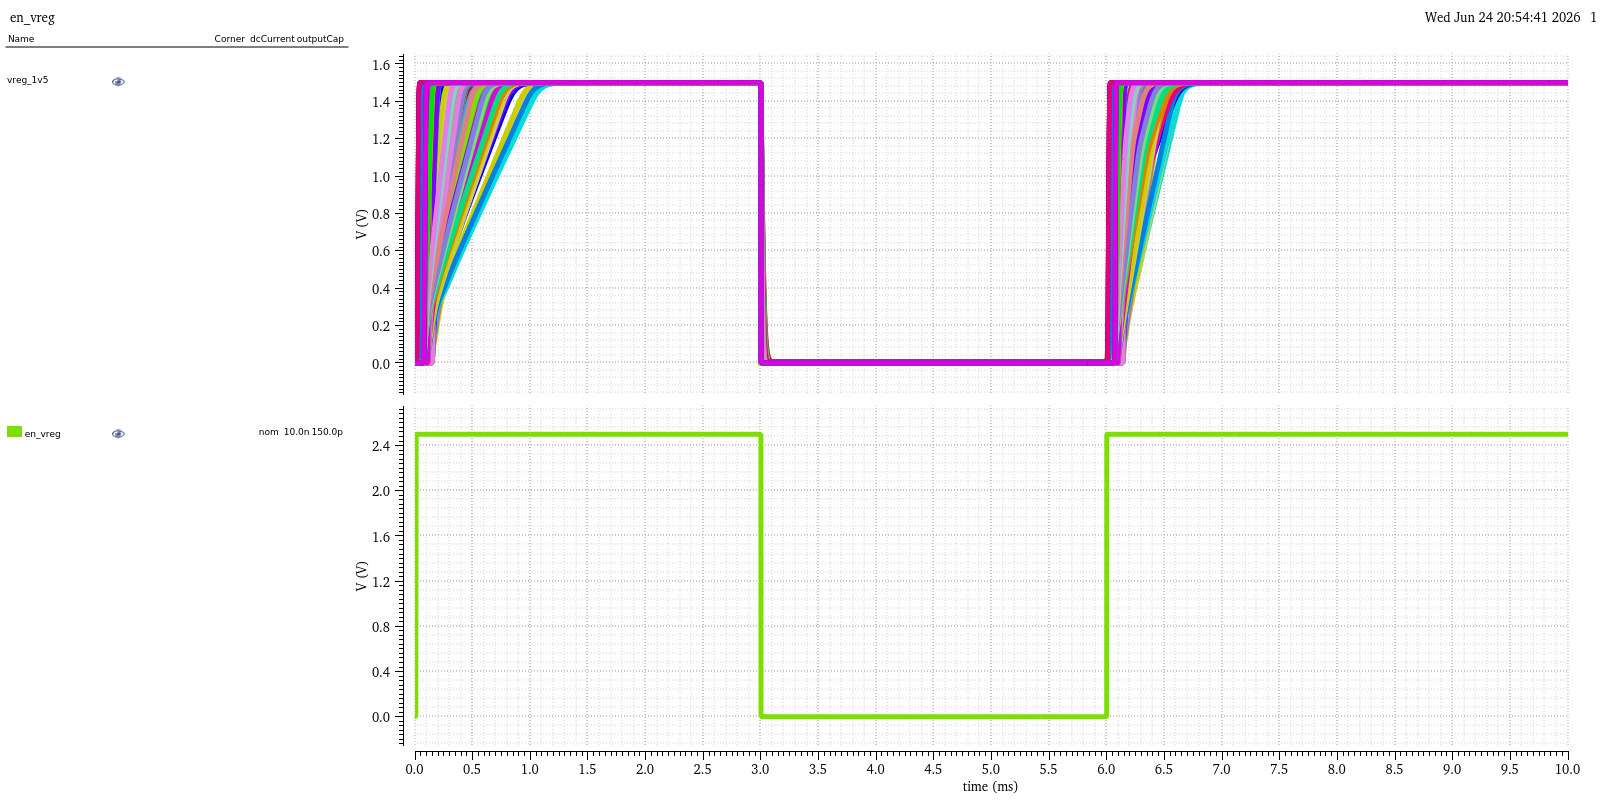
\includegraphics[keepaspectratio,alt={reg1v5 disable pvt cload 150p 5n 10n 10m sweep}]{../experimental_results/images/reg1v5_disable_pvt_cload_150p_5n_10n_10m_sweep.png}}
\caption{Disable Behaviour of the 1.5V Regulator over PVT with 150pF and
5nF Load Capacitance and Load Current Sweep from 10nA to
10mA}\label{reg1v5_disable_pvt_cload_150p_5n_10n_10m_sweep}
\end{figure}

The disable behaviour of the 1V5 Reg is also influenced by the load
current and load capacitance. The disable time is generally shorter than
the startup time, but it can still vary significantly depending on the
PVT conditions and the load current. The longest disable time is
observed when the load current is low (10nA) and the load capacitance is
large, as the pulldown switch needs to discharge the load capacitance
before it can fully disable.

\subsection{Static and Dynamic
Measurements}\label{_static_and_dynamic_measurements}

\begin{figure}
\centering
\pandocbounded{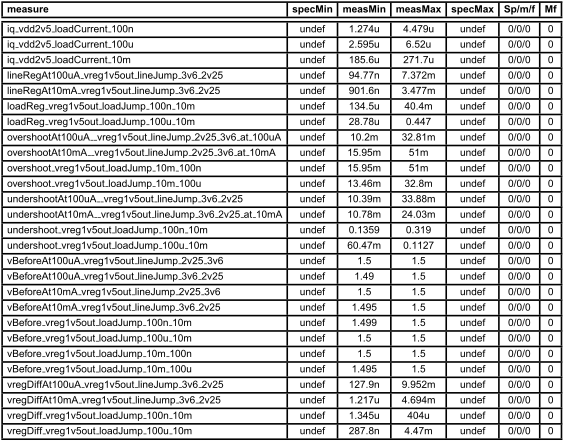
\includegraphics[keepaspectratio]{../experimental_results/images/loadAndLineJumpPlots/staticAndDynamicMeasurmentTable.pdf}}
\caption{Summary table that contains the minimum and maximum values of
the static and dynamic measurements for the 1.5V Regulator over PVT with
load capacitance swept between 150pF and
5nF}\label{staticAndDynamicMeasurmentTable}
\end{figure}

As can be seen from \hyperref[staticAndDynamicMeasurmentTable]{Summary
table that contains the minimum and maximum values of the static and
dynamic measurements for the 1.5V Regulator over PVT with load
capacitance swept between 150pF and 5nF}, the regulator manages to
achieve a maximum overshoot of 50mV for positive line jumps from 2.25V
to 3.6V at 10mA. The maximum undershoot for negative line jumps from
3.6V to 2.25V is 34mV at 10mA. As far as the load transient performance
is concerned, the maximum overshoot.

\subsubsection{Plots}\label{_plots}

\begin{figure}
\centering
\pandocbounded{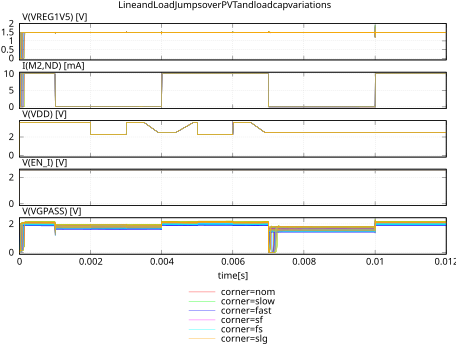
\includegraphics[keepaspectratio]{../experimental_results/images/loadAndLineJumpPlots/tran_loadAndLineJump_stackedPlot.pdf}}
\caption{}
\end{figure}

\begin{figure}
\centering
\pandocbounded{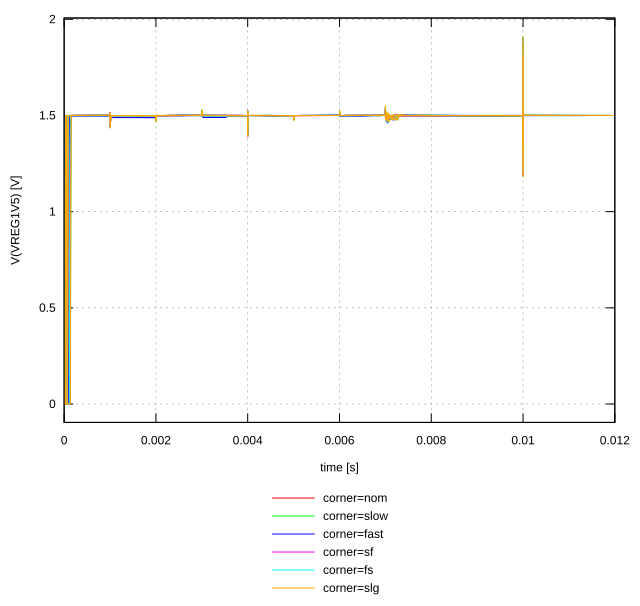
\includegraphics[keepaspectratio]{../experimental_results/images/loadAndLineJumpPlots/tran_loadAndLineJump_vreg1v5.pdf}}
\caption{}
\end{figure}

\begin{figure}
\centering
\pandocbounded{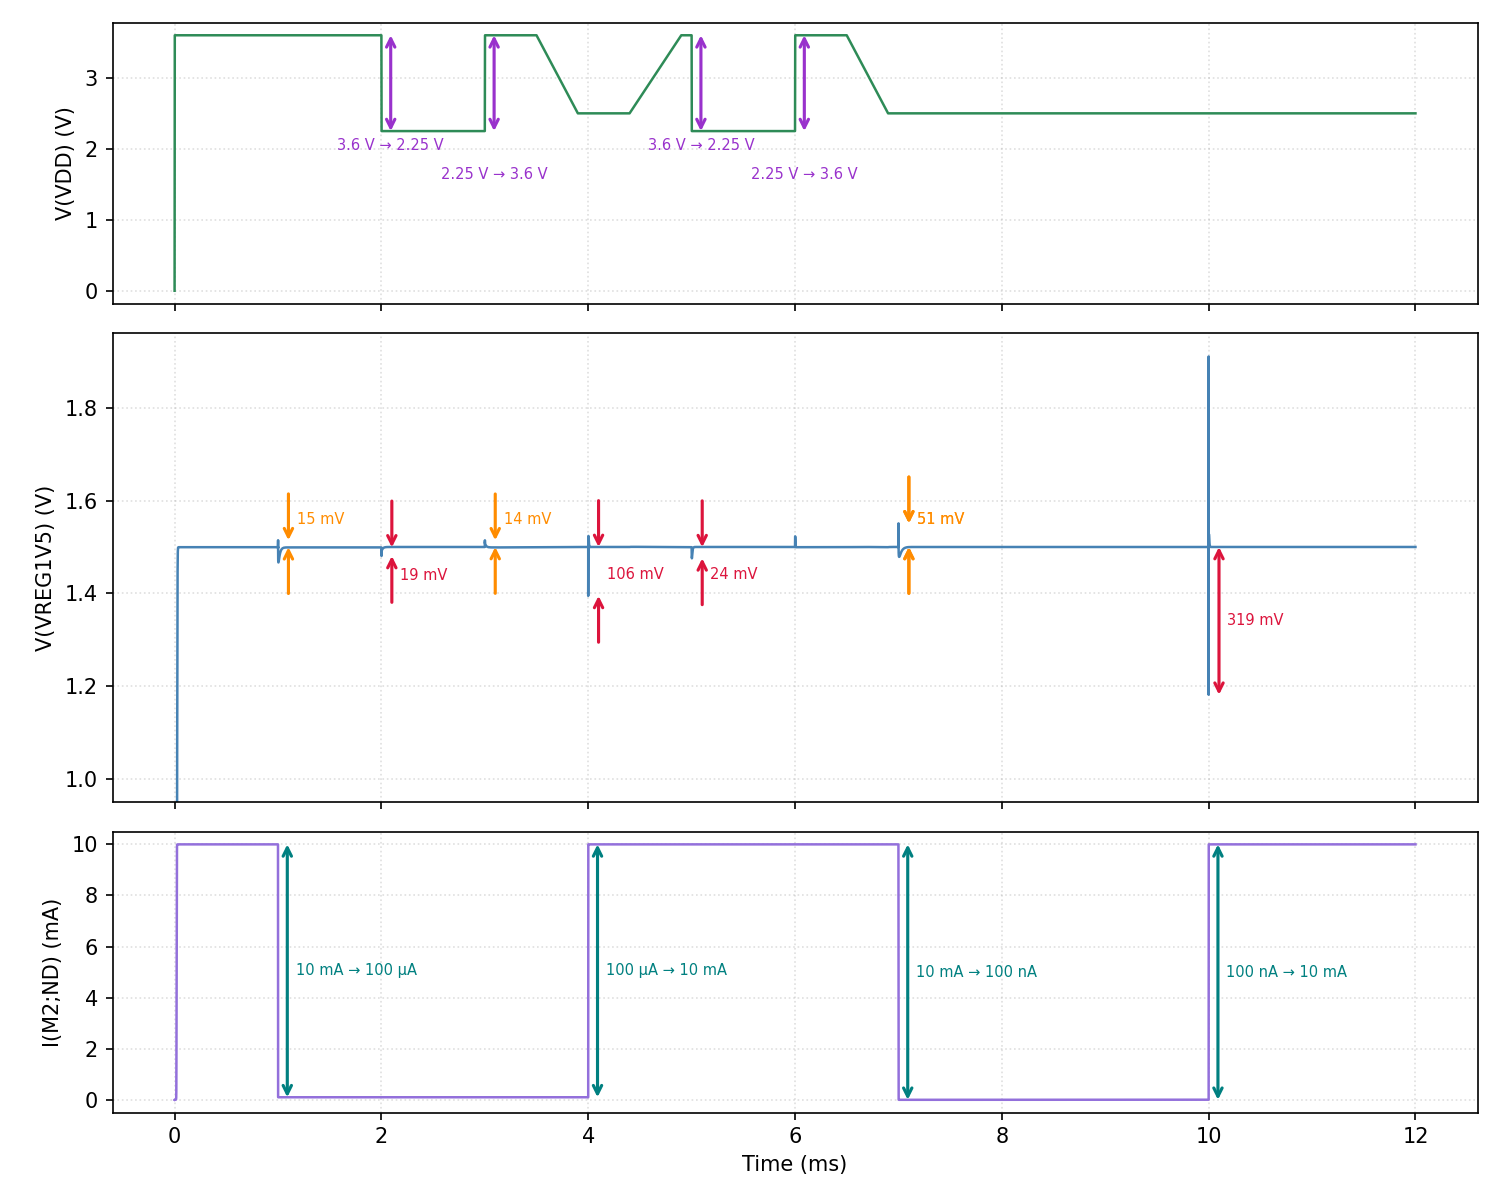
\includegraphics[keepaspectratio,alt={max overshoot vreg1v5out loadJump 10m 100n}]{../experimental_results/images/loadAndLineJumpPlots/max_overshoot_vreg1v5out_loadJump_10m_100n.png}}
\caption{Worst case corner for the 10mA to 100nA load jump
overshoot}\label{max_overshoot_vreg1v5out_loadJump_10m_100n}
\end{figure}

\begin{figure}
\centering
\pandocbounded{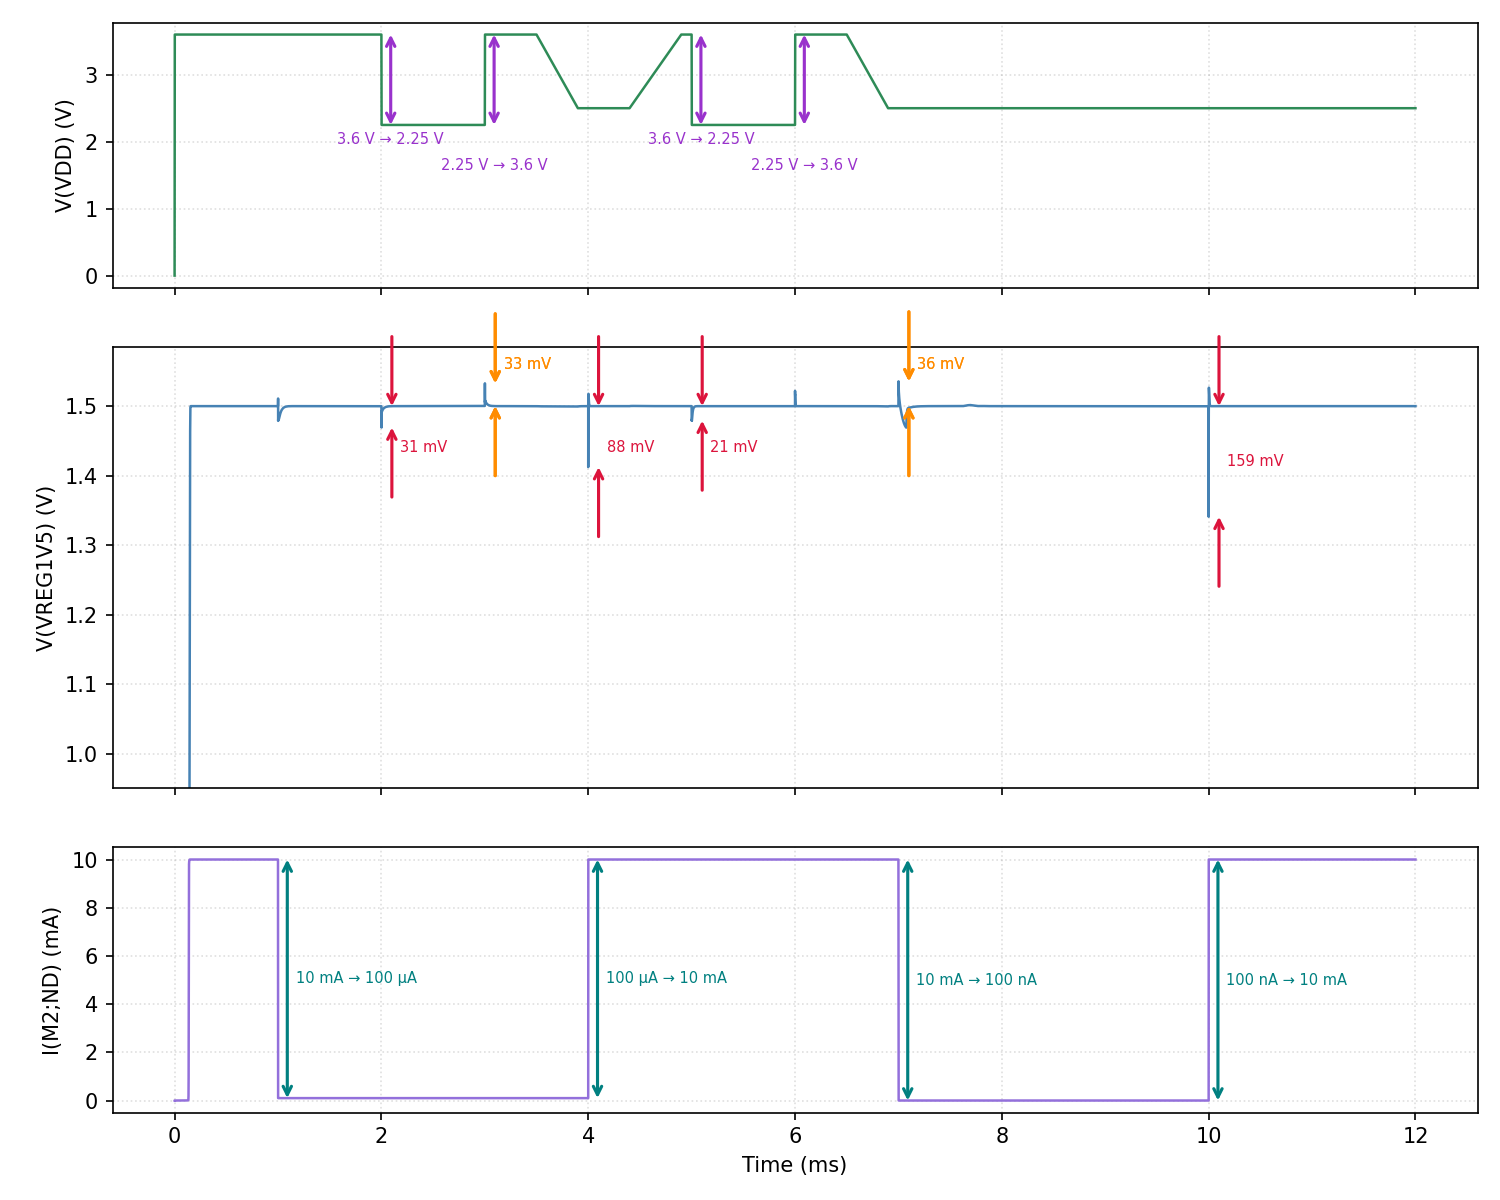
\includegraphics[keepaspectratio,alt={max overshoot vreg1v5out loadJump 10m 100u}]{../experimental_results/images/loadAndLineJumpPlots/max_overshoot_vreg1v5out_loadJump_10m_100u.png}}
\caption{Worst case corner for the 10mA to 100uA load jump
overshoot}\label{max_overshoot_vreg1v5out_loadJump_10m_100u}
\end{figure}

\begin{figure}
\centering
\pandocbounded{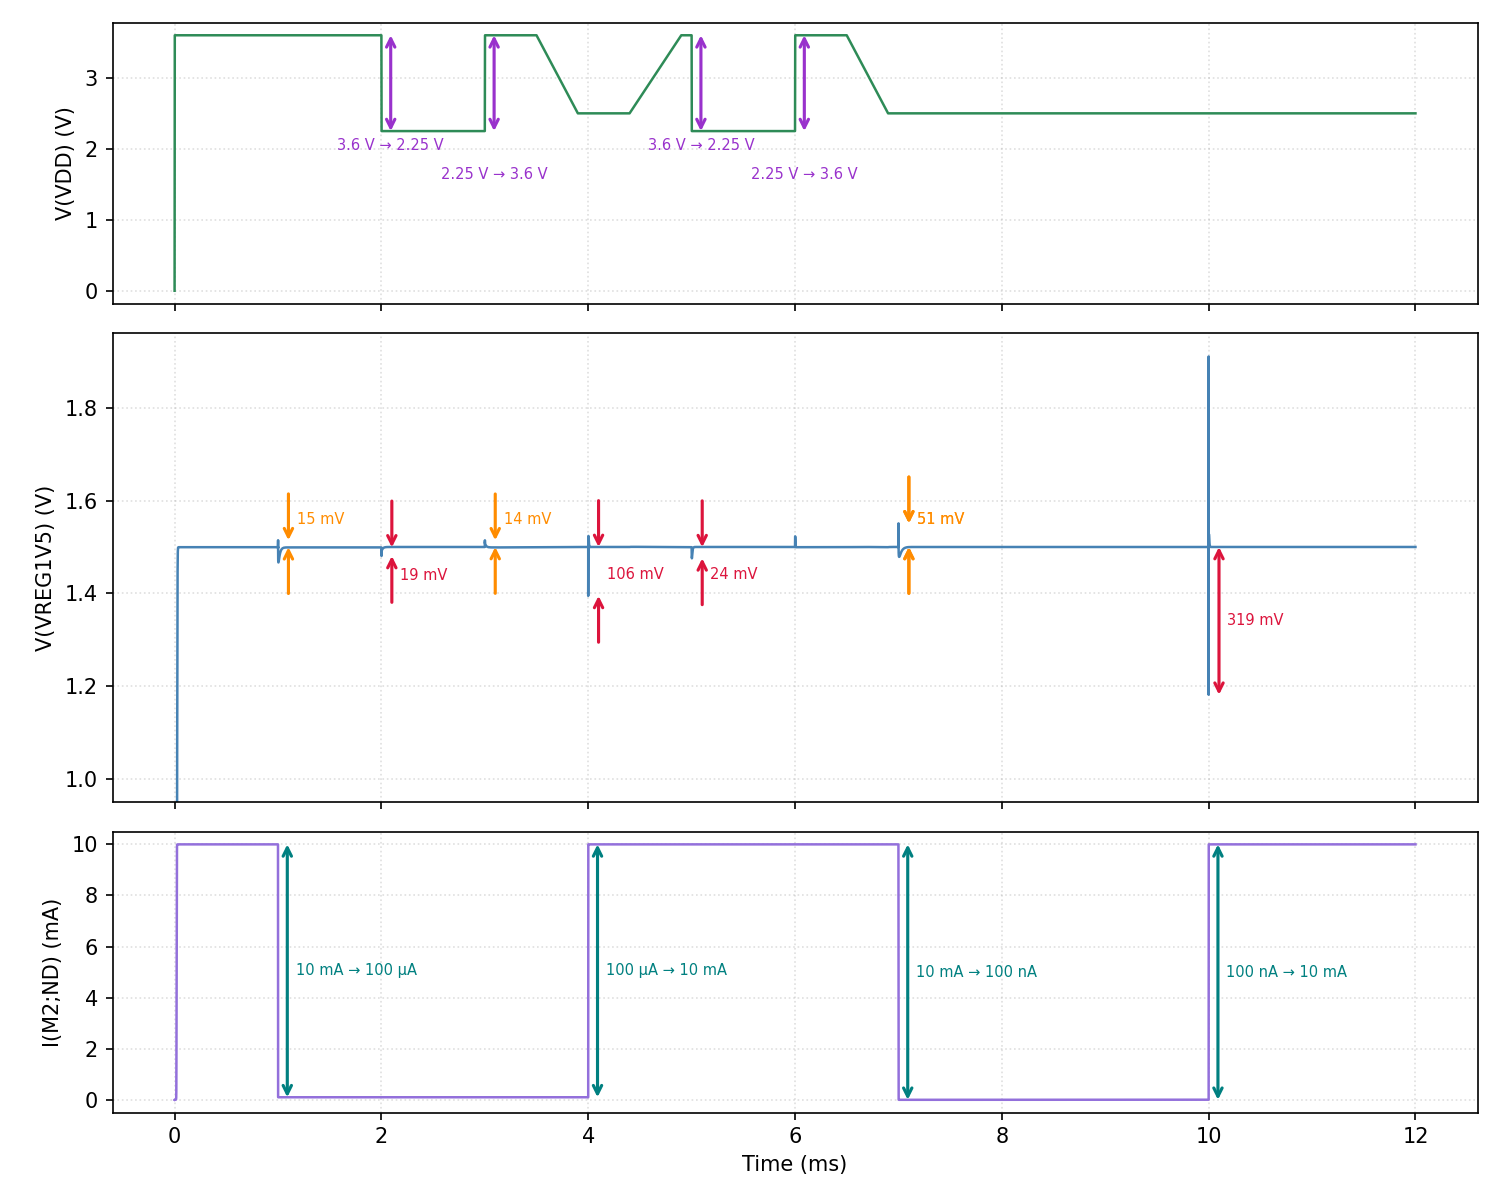
\includegraphics[keepaspectratio,alt={max overshootAt10mA vreg1v5out lineJump 2v25 3v6}]{../experimental_results/images/loadAndLineJumpPlots/max_overshootAt10mA__vreg1v5out_lineJump_2v25_3v6.png}}
\caption{Worst case corner for the 2.25V to 3.6V overshoot at 10mA load
current}\label{max_overshoot_vreg1v5out_loadJump_2_25v_3_6v}
\end{figure}

\begin{figure}
\centering
\pandocbounded{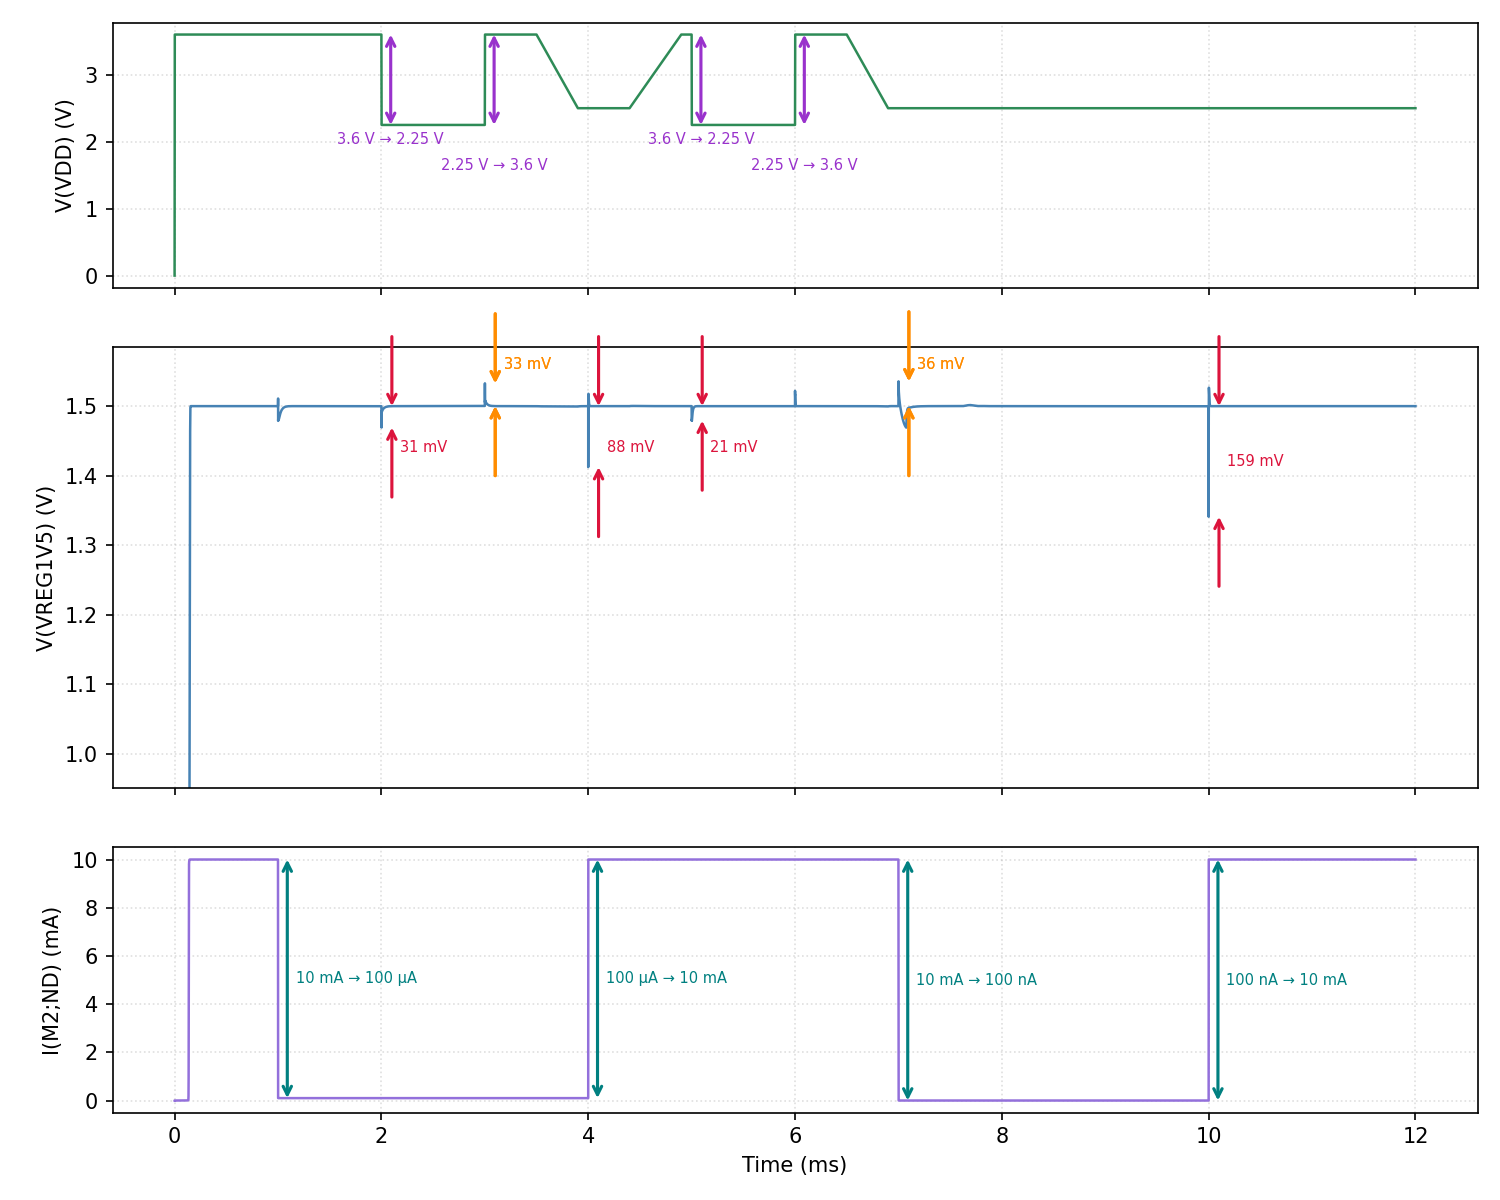
\includegraphics[keepaspectratio,alt={max overshootAt100uA vreg1v5out lineJump 2v25 3v6}]{../experimental_results/images/loadAndLineJumpPlots/max_overshootAt100uA__vreg1v5out_lineJump_2v25_3v6.png}}
\caption{Worst case corner for the 2.25V to 3.6V overshoot at 100uA load
current}\label{max_overshootAt100uA__vreg1v5out_lineJump_2v25_3v6}
\end{figure}

\begin{figure}
\centering
\pandocbounded{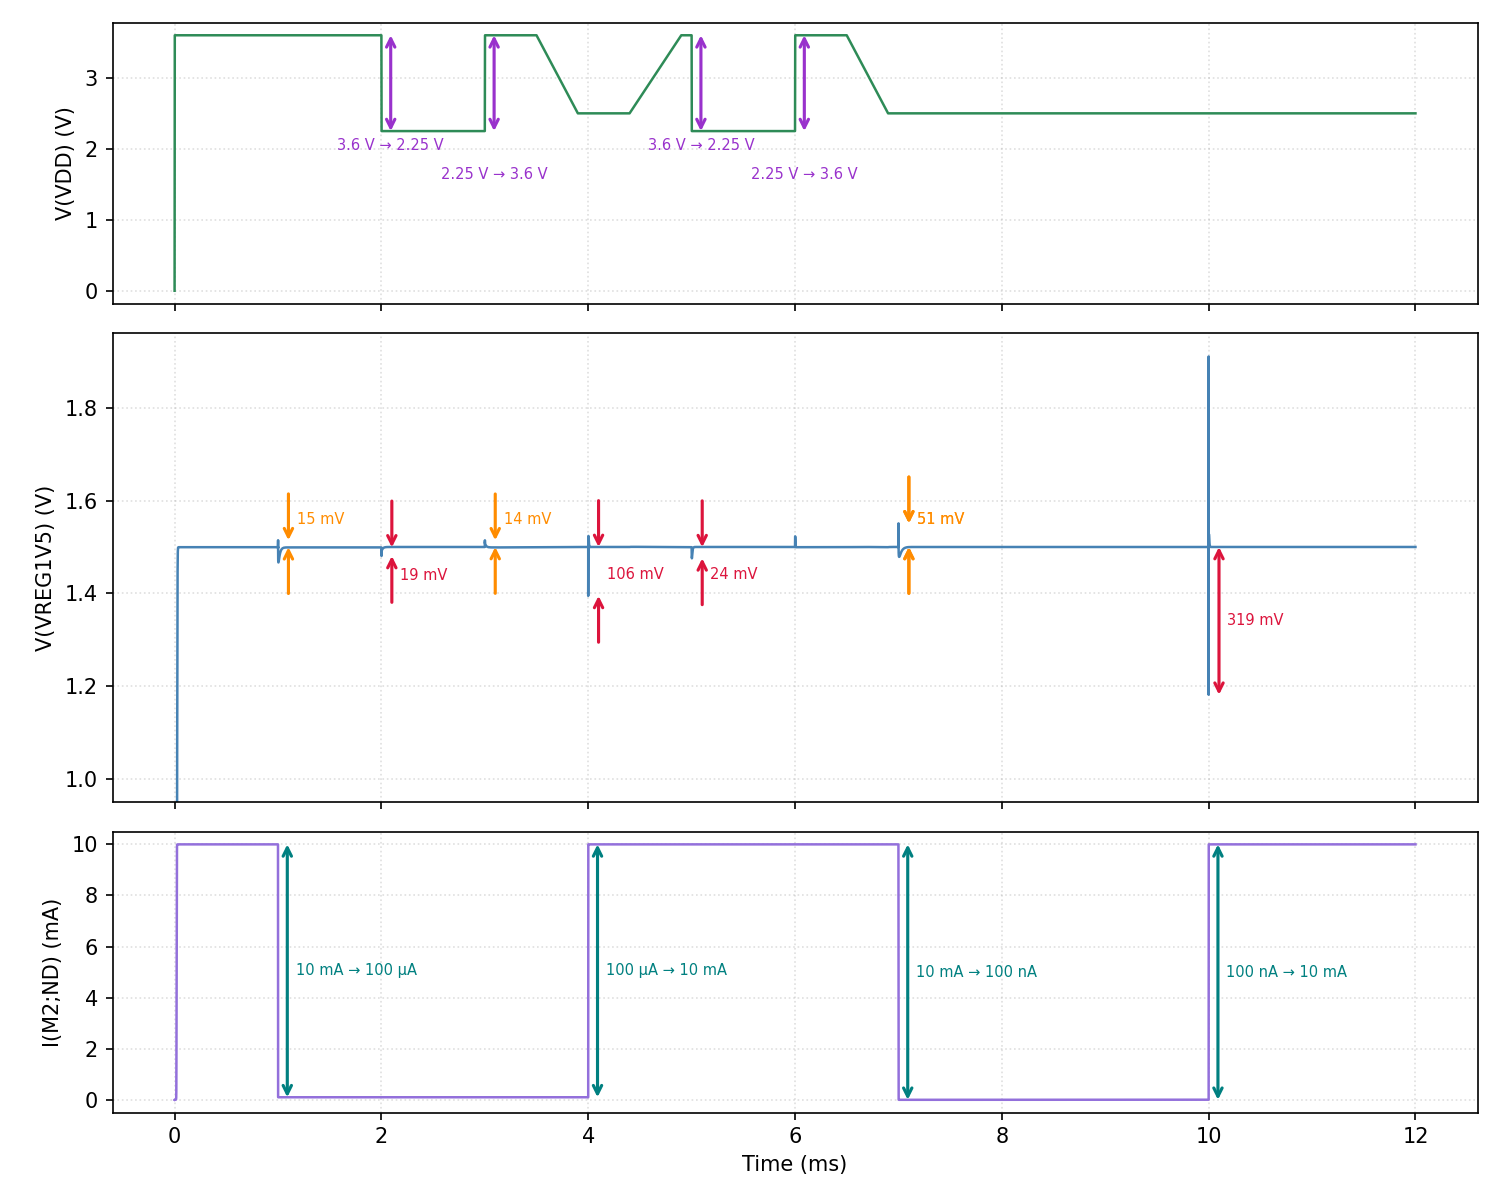
\includegraphics[keepaspectratio,alt={max undershoot vreg1v5out loadJump 100n 10m}]{../experimental_results/images/loadAndLineJumpPlots/max_undershoot_vreg1v5out_loadJump_100n_10m.png}}
\caption{Worst case corner for the 100nA to 10mA load jump
undershoot}\label{max_undershoot_vreg1v5out_loadJump_100n_10m}
\end{figure}

\begin{figure}
\centering
\pandocbounded{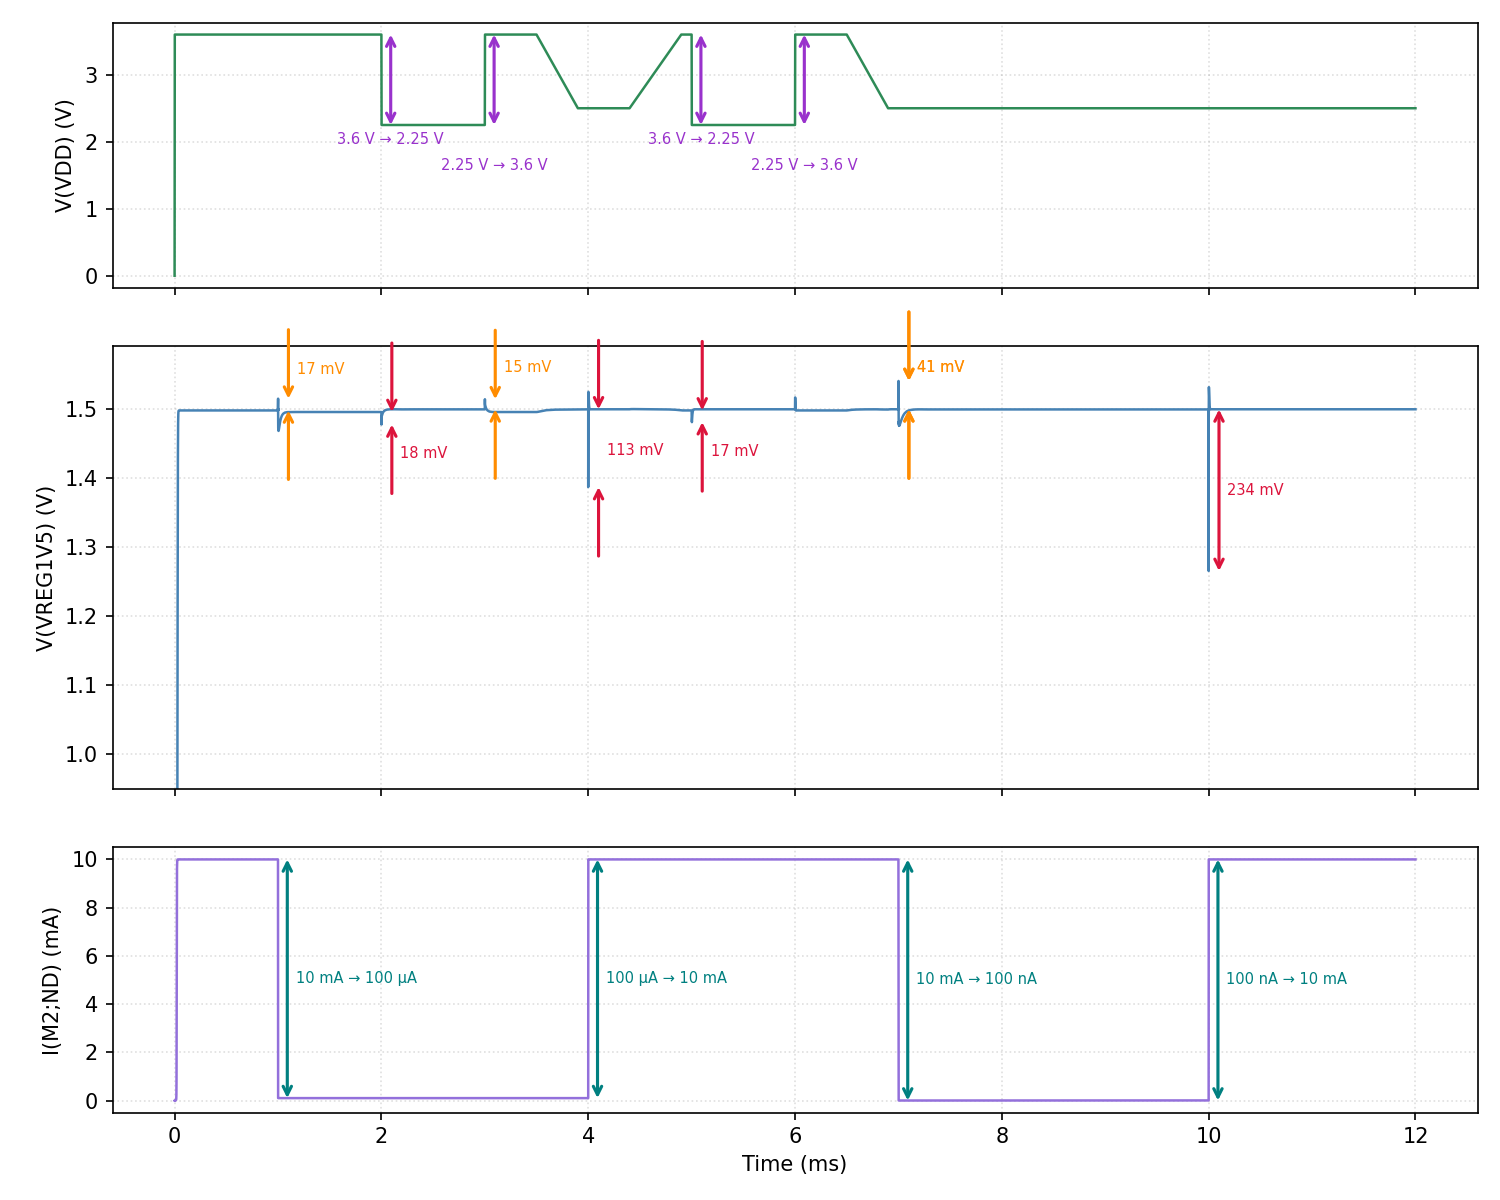
\includegraphics[keepaspectratio,alt={max undershoot vreg1v5out loadJump 100u 10m}]{../experimental_results/images/loadAndLineJumpPlots/max_undershoot_vreg1v5out_loadJump_100u_10m.png}}
\caption{Worst case corner for the 100uA to 10mA load jump
undershoot}\label{max_undershoot_vreg1v5out_loadJump_100u_10m}
\end{figure}

\begin{figure}
\centering
\pandocbounded{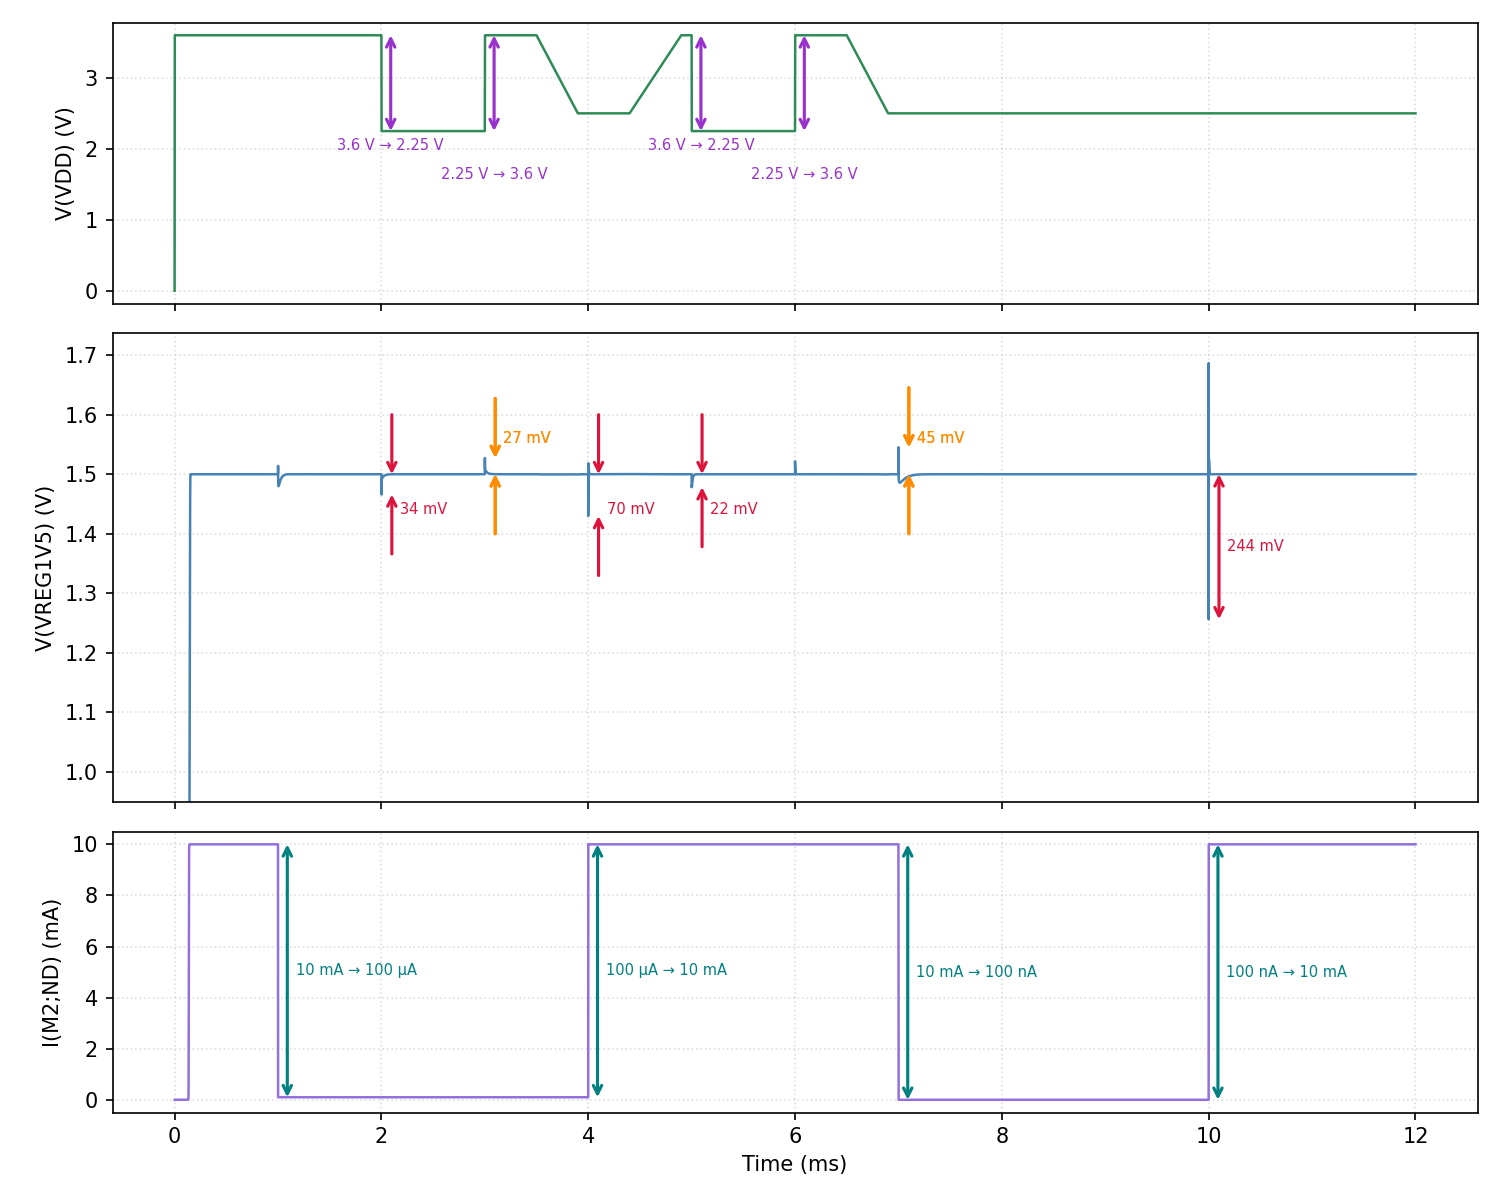
\includegraphics[keepaspectratio,alt={max undershootAt100uA vreg1v5out lineJump 3v6 2v25}]{../experimental_results/images/loadAndLineJumpPlots/max_undershootAt100uA__vreg1v5out_lineJump_3v6_2v25.png}}
\caption{Worst case corner for the 3.6V to 2.25V undershoot at 100uA
load current}\label{max_undershootAt100uA__vreg1v5out_lineJump_3v6_2v25}
\end{figure}

\begin{figure}
\centering
\pandocbounded{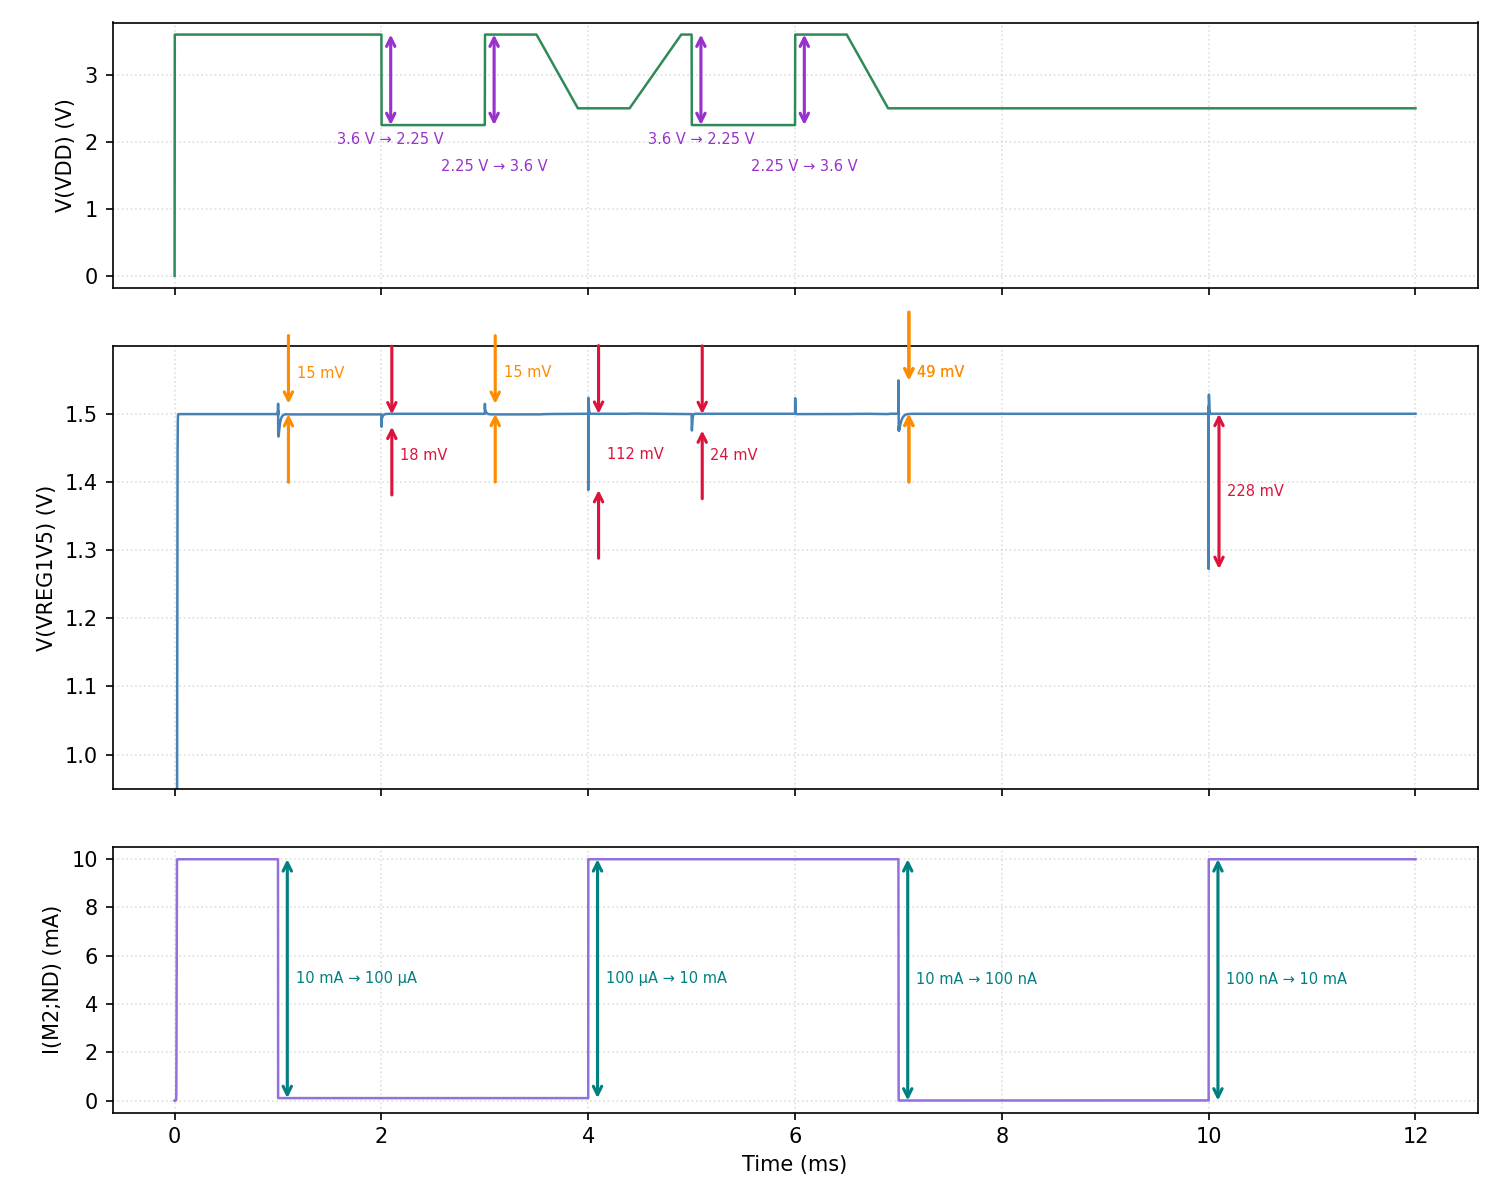
\includegraphics[keepaspectratio,alt={max undershootAt10mA vreg1v5out lineJump 3v6 2v25}]{../experimental_results/images/loadAndLineJumpPlots/max_undershootAt10mA__vreg1v5out_lineJump_3v6_2v25.png}}
\caption{Worst case corner for the 3.6V to 2.25V undershoot at 10mA load
current}\label{max_undershootAt10mA__vreg1v5out_lineJump_3v6_2v25}
\end{figure}

\subsection{PSRR}\label{_psrr}

\begin{figure}
\centering
\pandocbounded{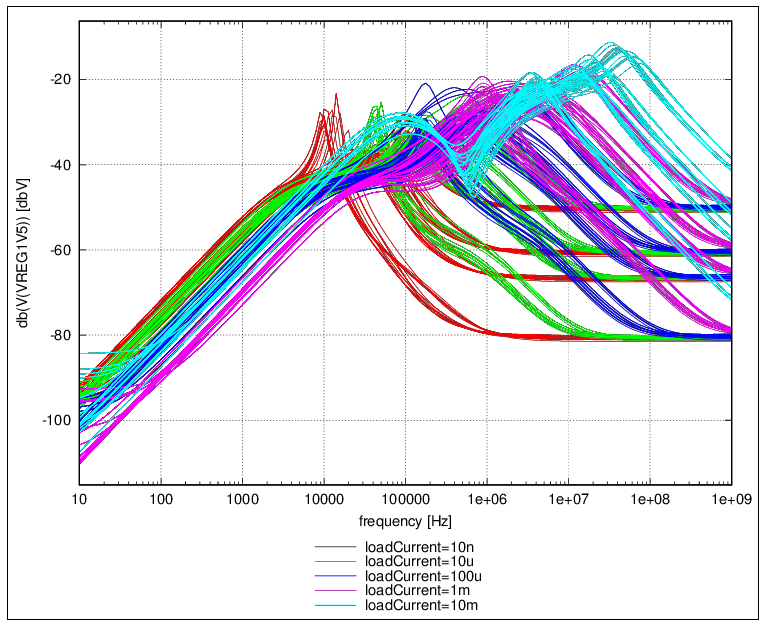
\includegraphics[keepaspectratio,alt={psrr plots over pvt}]{../experimental_results/images/psrr_plots_over_pvt.png}}
\caption{}
\end{figure}

The regulator's PSRR maintains its worst case value over a frequency
band of 10 Hz to 1GHz of under -13dB even at the maximum load current.
Also because of the high open loop DC gain, it manages to have a maximum
low frequency PSRR value of under -70dB at 100Hz.

\begin{figure}
\centering
\pandocbounded{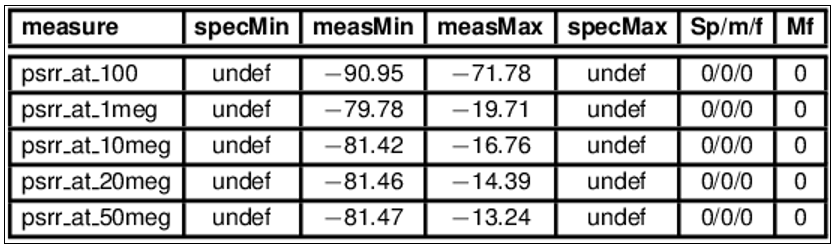
\includegraphics[keepaspectratio,alt={psrr pvt measurements}]{../experimental_results/images/psrr_pvt_measurements.png}}
\caption{}
\end{figure}

\end{document}